\documentclass[12pt]{article}
\usepackage{float}
\usepackage{amsthm}
\usepackage{amsmath}
\usepackage{lineno}
\usepackage{cite}
\usepackage{amssymb,graphics,color,cite,amsmath}
\usepackage{subfig}
\usepackage{graphicx}
\usepackage{epsfig}
\usepackage{psfrag}
\usepackage[margin=0.75in]{geometry}
\usepackage{float}
\usepackage{afterpage}
\usepackage{hyperref}
\usepackage{verbatim}

\usepackage[noblocks]{authblk}
%\usepackage{natbib}
\usepackage{stackengine}

\usepackage{xspace}
\newcommand{\themename}{\textbf{\textsc{metropolis}}\xspace}

\renewcommand{\(}{\left (}
\renewcommand{\)}{\right )}
\renewcommand{\vec}[1]{\boldsymbol{#1}}

\begin{document}

\title{A Series of Experiments Based on Gyroscope}
\date{}
\author[1]{Zeshun Zong}
\author[2]{Yifeng Chen}
\affil[1,2]{\footnotesize Courant Institute of Mathematical Sciences, New York University, New York}


\maketitle
\begin{abstract}
Using Rigid Body Motion, we built a model to simulate the motion of gyroscope. We analyzed the motion of a single gyroscope under different with uneven mass distributions. We stacked a few gyroscopes vertically and from our experiment we see that hardly can the combination rotate stably. Moreover, we studied the physics behind gyrocompass and successfully simulated how it works. Some basic properties of gyrocompass are also discussed.
\end{abstract}

\section{Introduction}

\hspace{5mm} In this project, we first consider a system that consists of one gyroscope. We will examine how the mass distribution and angular momentum affects the trace of the top node. We then move on to a more complex system that consists of more than one gyroscope and observe its behavior.

Another subject of interest is the application of gyroscopes in inertial guidance systems. In a simple gyrocompass model, a gyroscope is mounted on a frame that is tangent to Earth's surface. Due to Earth's rotation, the axis of rotation will gradually point to true North. However, the axis of rotation doesn't stay in the true North direction. In fact, it keeps oscillating between a small angle. The goal of this project is to build a model of the gyro-compass and study the relation between the gyroscope's angular velocity and its angle of oscillation.


\section{Preliminaries: Rigid Body Motion}
\hspace{5mm} Here we introduce some important concepts related to the rigid body motion. In physics, a rigid body motion can always be decomposed into a translation and a rotation about its center of mass. As is shown in Figure 1, a force is applied on one end of a pole. Assuming that the force is acting the center of mass, we will get a translation which is governed by Newton's Second Law, $\vec{F} = m\vec{a},$ where $\vec{F}$ is the force, $m$ is the mass of the object, and $\vec{a}$ is its tranlational acceleration. Or equivalently,
\begin{equation}
{\vec{F}} = m \cdot \frac{d\vec{u}}{dt},
\end{equation} where $\vec{u}$ is the velocity of the center of mass.
\\
\begin{figure}[ht]

		\centering
		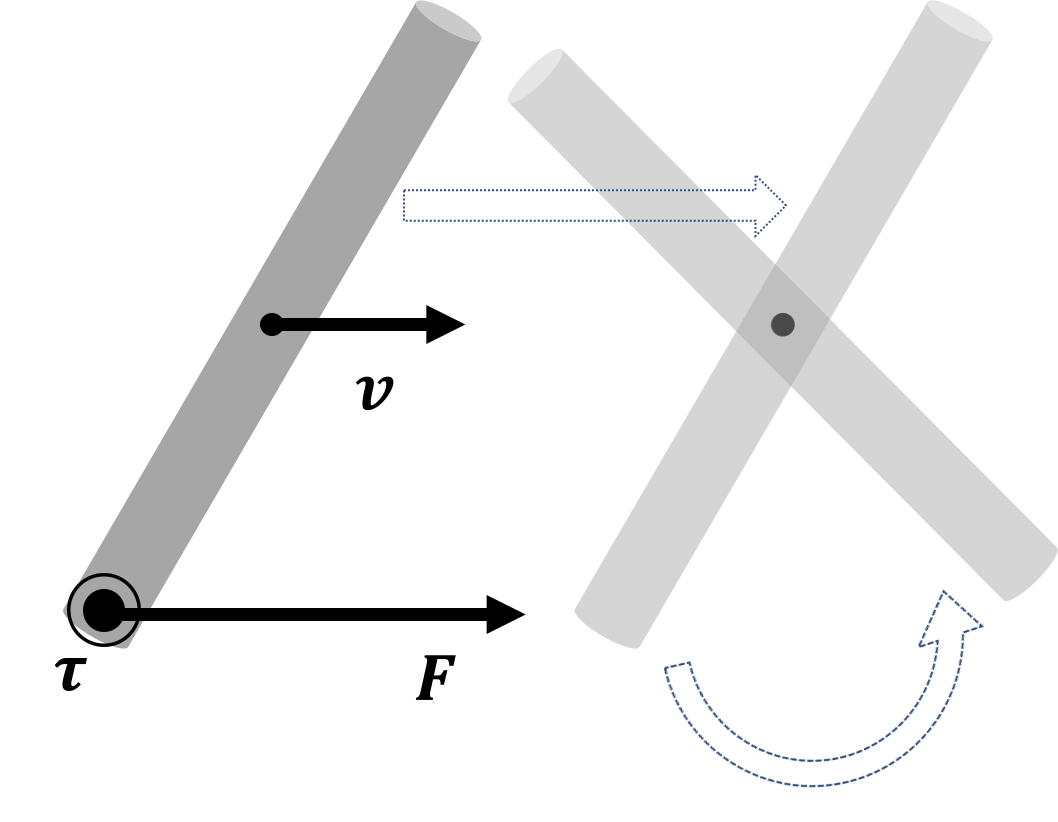
\includegraphics[width=0.33\textwidth]{prelim_demo.png}
		\caption*{\small Figure 1}

\end{figure}

The force $\vec{F}$ will also yield a torque $\vec{\tau}$ to the object. Torque can be thought as of a twist to an object, which is defined to be $$\vec{\tau} = \vec{r} \times \vec{F},$$ where $\vec{r}$ is the position vector of the point on which the force is applied. The magnitude of torque shows how large the twist is, and the direction of torque is the direction of rotation that the twist generates (right hand rule). In our graph, the rotation is clock-wise, so by the right hand rule, $\vec{\tau}$ is pointing inward. The rotation is described by angular momentum $\vec{L}.$ It is a vector whose length describes how fast the rotation is, and whose direction describes the direction of rotation by right hand rule. Angular momentum is defined to be $$\vec{L} = I\vec{\Omega},$$ where $I$ is moment of inertia, which describes the distribution of masses on the object, and $\vec{\Omega}$ is angular velocity. Angular momentum is conservative unless torque is exerted, and the rotation is governed by
\begin{equation}
\frac{d\vec{L}}{dt} = \vec{\tau}.
\end{equation}
\hspace{5mm} Equations (1) and (2) together define a rigid body motion: a motion of an object is simply a translation of its center of mass and a rotation about its center of mass, i.e. for a particular point $k$ on the object, its velocity is \begin{equation}
\vec{u}_k (t) = \vec{u_{cm}} (t) + \vec{\Omega}(t) \times \vec{r_k},
\end{equation} where $\vec{u_{cm}}$ is the translational velocity of the center of mass.



\section{Mathematical Modeling}
\subsection{Basic Model}

\hspace{5mm} Following the above physical equations that determine a rigid body motion, we hereby setup a general model for implementation. We view a rigid body as a set of mass points (nodes) connected by links. Only external forces are considered, and internal forces between nodes are not considered (even if we discuss internal forces, they will cancel out due to Newton's Third Law and will not influence the motion of the object). Let subscript $k$ denote the $k^{th}$ node. Let subscript $cm$ denote the center of mass. Let $\vec{X_k}$ denote the position of node $k$, $\vec{U_k}$ the velocity of node $k$, and $m_k$ the mass of node $k.$ By definition of angular momentum, \begin{equation}
    \vec{L}(t) = \sum_k m_k (\vec{X_k} - \vec{X_{cm}}) \times (\vec{U_k} - \vec{U_{cm}}) = \sum_k m_k (\vec{X_k} - \vec{X_{cm}}) \times \vec{U_k}.
\end{equation}
The second equality follows from the definition of center of mass.

Differentiate both sides with respect to $t,$
\begin{align}
	\frac{d\vec{L}(t)}{dt} &= \sum_k (\vec{X_k}(t) - \vec{X_{cm}}(t)) \times m_k \frac{d\vec{U_k}(t)}{dt}\\
	&=\sum_k (\vec{X_k}(t) - \vec{X_{cm}}(t)) \times m_k \frac{d\vec{U_k}(t)}{dt} - \{\sum_k m_k (\vec{X_k}(t)- \vec{X_{cm}}(t)) \} \times \frac{d\vec{U_{cm}}(t)}{dt} \\
	&=\sum_k (\vec{X_k}(t) - \vec{X_{cm}}(t)) \times m_k \frac{d\vec{U_k}(t)}{dt}\\
	&= \sum_k (\vec{X_k}(t) - \vec{X_{cm}}(t)) \times \vec{F_k}(t) \\
	&= \sum_k \vec{\widetilde{X_k}}(t) \times \vec{F_k}(t),
\end{align}
where $\vec{F_k}$ denotes the external force acting on this node, and $\vec{\widetilde{X_k}} = \vec{X_k} - \vec{X_{cm}}$ is the positional vector of this node. The fourth equality follows from Newton's Second Law.

Now we have two equations that completely describe a rigid body motion, namely
\begin{equation}
	M \frac{d\vec{U_{cm}}(t)}{dt} = \sum_k \vec{F_k}(t),
\end{equation}
where $M = \sum_k m_k$ is the total mass, and \begin{equation}
\frac{d\vec{L}(t)}{dt} = \sum_k \vec{\widetilde{X_k}}(t) \times \vec{F_k}(t).
\end{equation}

Since we want the motion to be rigid, it is important that we can solve for the angular velocity. Notice that the general form of motion of the $k^{th}$ node is given by equation (3). Substituting this into (4), we see that
\begin{align}
	\vec{L}(t) &= \sum_k m_k \vec{\widetilde{X_k}}(t) \times (\vec{\Omega}(t) \times \vec{\widetilde{X_k}}(t)) \\
	&= \{\sum_k m_k |\vec{\widetilde{X_k}}(t)|^2\}\vec{\Omega}(t) - \sum_k m_k \vec{\widetilde{X_k}}(t)(\vec{\widetilde{X_k}}(t)\cdot \vec{\Omega}(t))\\
	&= \{\sum_k m_k [|\vec{\widetilde{X_k}}(t)|^2 E - \vec{\widetilde{X_k}} \cdot \vec{\widetilde{X_k}}^T ]\} \vec{\Omega} \\
	&= {I}(t) \vec{\Omega}(t),
\end{align}
where we let $I(t)$, the moment of inertia, denote $\sum_k m_k [|\vec{\widetilde{X_k}}(t)|^2 E - \vec{\widetilde{X_k}} \cdot \vec{\widetilde{X_k}}^T ].$ Here $E$ stands for the identity matrix. We see that the expression for $I(t)$ does conform with the definition the moment of inertia.

Notice that a nice property of $I$, the moment of inertia matrix is that it is positive definite as long as the object has some width. So we can solve for $\vec{\Omega}$ simply by \begin{equation}
\vec{\Omega}(t) = I(t)^{-1}\vec{L}(t).
\end{equation}

Given $\vec{\Omega}(t),$ the angular velocity, we would like to construct a rotation matrix $\vec{R}(\vec{\Omega}(t), \Delta t)$ (which is an orthogonal matrix) that performs the exact rotation. To be more specific, $\vec{R}$ rotates every position vector about the rotating axis for an angle $\vec{\Omega}(t)\Delta t$ (we assume that within the $\Delta t$ period of time, the angular velocity is constant).

Below we dropped the time $t$ for conciseness. The part of the vector that will not be affected by the rotation is its projection onto the unit vector in the direction of $\vec{\Omega}$, namely:
\begin{equation}
\frac{\vec{\Omega}}{\|\vec{\Omega}\|} \frac{\vec{\Omega}^T}{\|\vec{\Omega}\|} \widetilde{\vec{X}} = {P}(\vec{\Omega}) \widetilde{\vec{X}}.
\end{equation}
Expressing
\begin{equation}
\widetilde{\vec{X}} = {P}(\vec{\Omega}) \widetilde{\vec{X}} + (E - {P}(\vec{\Omega})) \widetilde{\vec{X}},
\end{equation}

We can see that the part of $\widetilde{\vec{X}}$ we need to rotate is $(E - {P}({\vec{\Omega}})) \widetilde{\vec{X}}.$  Here $E$ is the identity matrix. Using this vector we construct a basis for the plane normal to $\vec{\Omega}$ and through the origin:
\begin{align}
    \vec{v}_1 &=  (E - P({\vec{\Omega}})) \widetilde{\vec{X}}, \\
\vec{v}_2 &=  \frac{\vec{\Omega}}{\|\vec{\Omega}\|} \times (E - {P}(\vec{\Omega})) \widetilde{\vec{ X}} = \frac{\vec{\Omega}}{\|{\vec{ \Omega}}\|} \times \widetilde{\vec{X}}.
\end{align}
 Notice that this basis $\{\vec{v}_1, \vec{v}_2\}$ is not necessarily orthonormal, so we need to normalize the two vectors. In the following discussion we assume $\{\vec{v}_1, \vec{v}_2\}$ is a set of orthonormal basis.  Now any vector $\vec{v}$ in this plane can be expressed as a linear combination of
\begin{equation}
    \vec{v} = \alpha_1 \vec{v}_1 + \alpha_2 \vec{v}_2.
\end{equation}


In particular, the basis vector $\vec{v}_1$, rotated by an amount $\|\vec{ \Omega}\|\Delta t$, can be written as
\begin{equation}
 \cos(\|\vec{\Omega}\|\Delta t)\vec{v}_1 + \sin(\|\vec{\Omega}\|\Delta t)\vec{v}_2.
\end{equation}
This rotated vector is precisely the part of $\widetilde{\vec{X}}$ which  rotates about the center of mass. The orthogonal matrix can be expressed as:
\begin{align}
{\vec{R}}(\vec{\Omega}, \Delta t) \widetilde{\vec{X}} = {P}({\vec{\Omega}}) \widetilde{\vec{X}} +  \cos(\|{\vec{ \Omega}}\|\Delta t) (E - { P}({\vec{ \Omega}})) \widetilde{\vec{X}} + \sin(\|{\vec{\Omega}}\|\Delta t) \frac{{\vec{\Omega}}}{\|{\vec {\Omega}}\|} \times \widetilde{\vec{X}}.
\end{align}

Finally we have everything needed to perform a timestep. We use forward Euler's method to do so. Given $\vec{X_k}(t), \vec{X_{cm}}(t), \vec{\widetilde{X_k}}(t), \vec{U}(t), \vec{U_{cm}}(t),$ and
$\vec{L}(t),$

\begin{itemize}

\item given $\widetilde{\vec{X}}_k(t)$, compute ${I}(t)$.
\item solve the system ${I}(t){\vec{\Omega}}(t) = \vec{ L}(t)$ for $\vec{\Omega}(t)$.
\item using $\vec{\Omega}(t)$, update $\widetilde{\vec{X}}_k(t + \Delta t) = \vec{R}({\vec{\Omega}}(t), \Delta t)\, \widetilde{\vec{X}}_k(t)$.
\item update the center of mass: $\vec{X_{cm}}(t + \Delta t) = \vec{ X_{cm}}(t) + \Delta t  \vec{U_{cm}}(t)$.
\item update the velocity of the center of mass:
\begin{equation*}
M \frac{\vec{U_{cm}}(t + \Delta t) - \vec{U_{cm}}(t)}{\Delta t} = \sum_k \vec{F_k}(t + \Delta t).
\end{equation*}
\item update the positions of the individual masses:
\begin{equation*}
\vec{X_k}(t+\Delta t) = \vec{X_{cm}}(t + \Delta t) + \widetilde{\vec{X_k}}(t+\Delta t)
\end{equation*}
\item update the angular momentum:
\begin{equation*}
    \frac{\vec{L}(t + \Delta t) - \vec{L}(t)}{\Delta t} = \sum_k \widetilde{\vec{X_k}}(t + \Delta t) \times \vec{F_k}(t + \Delta t).
\end{equation*}


\end{itemize}


\subsection{A Simple Gyroscope}
\hspace{5mm} In a simple gyroscope model, there are only three forces acting on the system: gravity, normal force and friction.
Gravity is applied to each node independently, while the normal force and friction are only applied on the bottom of the axis. See figure 2.

There are a few ways to simulate the normal force. Here, the simulation is achieved by adding a surface z=0, which represents the ground. The gyroscope receives a normal force pointing vertically upward when the bottom node sinks below the surface, and zero when the node is above the surface. When the bottom node is below the surface z=0, we model the normal force by setting its magnitude proportional to distance between the bottom node and the ground. The coefficient represents the stiffness or the ground.

Friction is not essential to the system. However, without the presence of friction, the total force applied on the gyroscope is the sum of gravity and normal force, which is zero on average. As a result, the center of mass will have very little movement and the bottom node will move in a circular path. In order the simulate the real world behavior of a gyroscope on the ground, we add friction to the system. The direction of the friction is inverse to that of the movement of the bottom node and the magnitude is computed by multiplying a friction coefficient to the normal force.
\begin {figure}[ht]
	\centering
    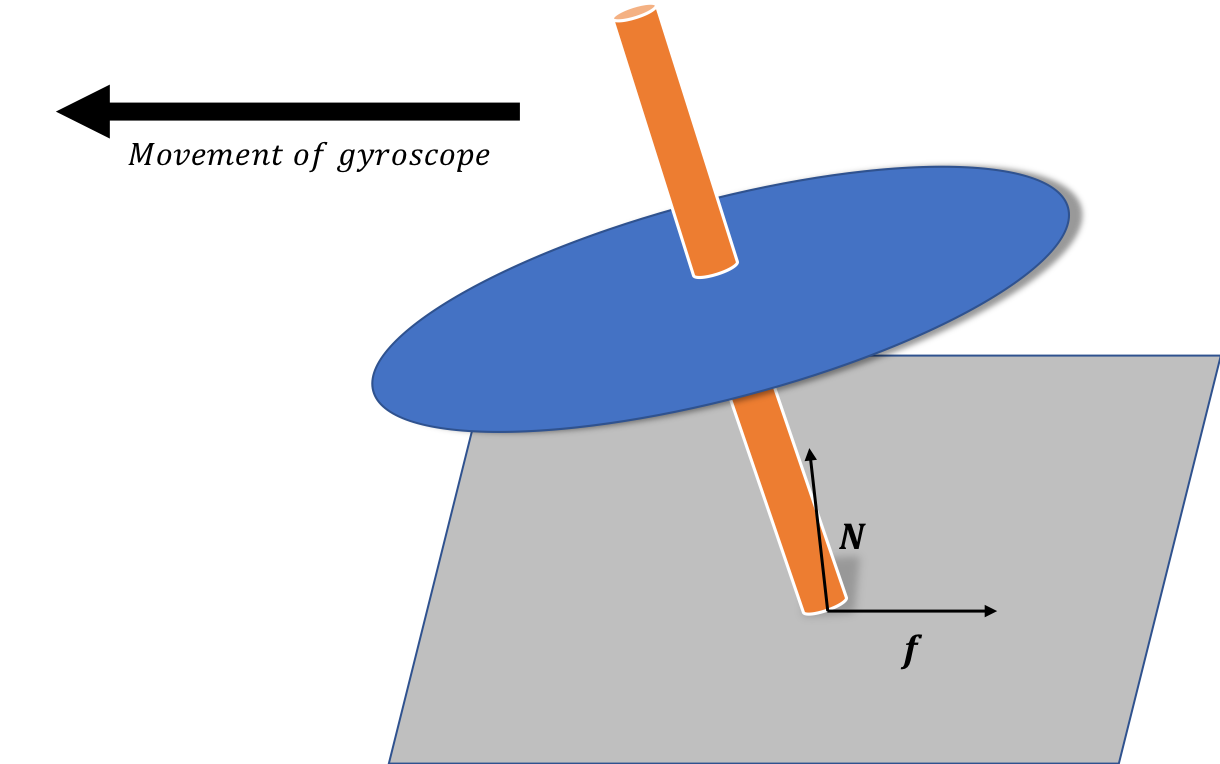
\includegraphics[width=0.5\textwidth]{1st_model.png}
    \caption*{\small Figure 2}
\end {figure}

This model is used to test the relation between the mass distribution and starting angular momentum of a gyroscope and its stability. Results are shown in section 4.1.

\subsection{Stack of Gyroscopes}
\hspace{5mm} In this model, we stack a few gyroscopes on top of each other to study the stability of this system. Each adjacent pair of gyroscopes are connected by a spring of rest length zero. See figure 3. Like the simple case model, we also have normal force and friction in the system. And they only act on the bottom node of the bottom gyroscope. Note that although in the graph below, each spring has a positive length, in our code, this rest length is set to be 0.
\begin {figure}[ht]
	\centering
    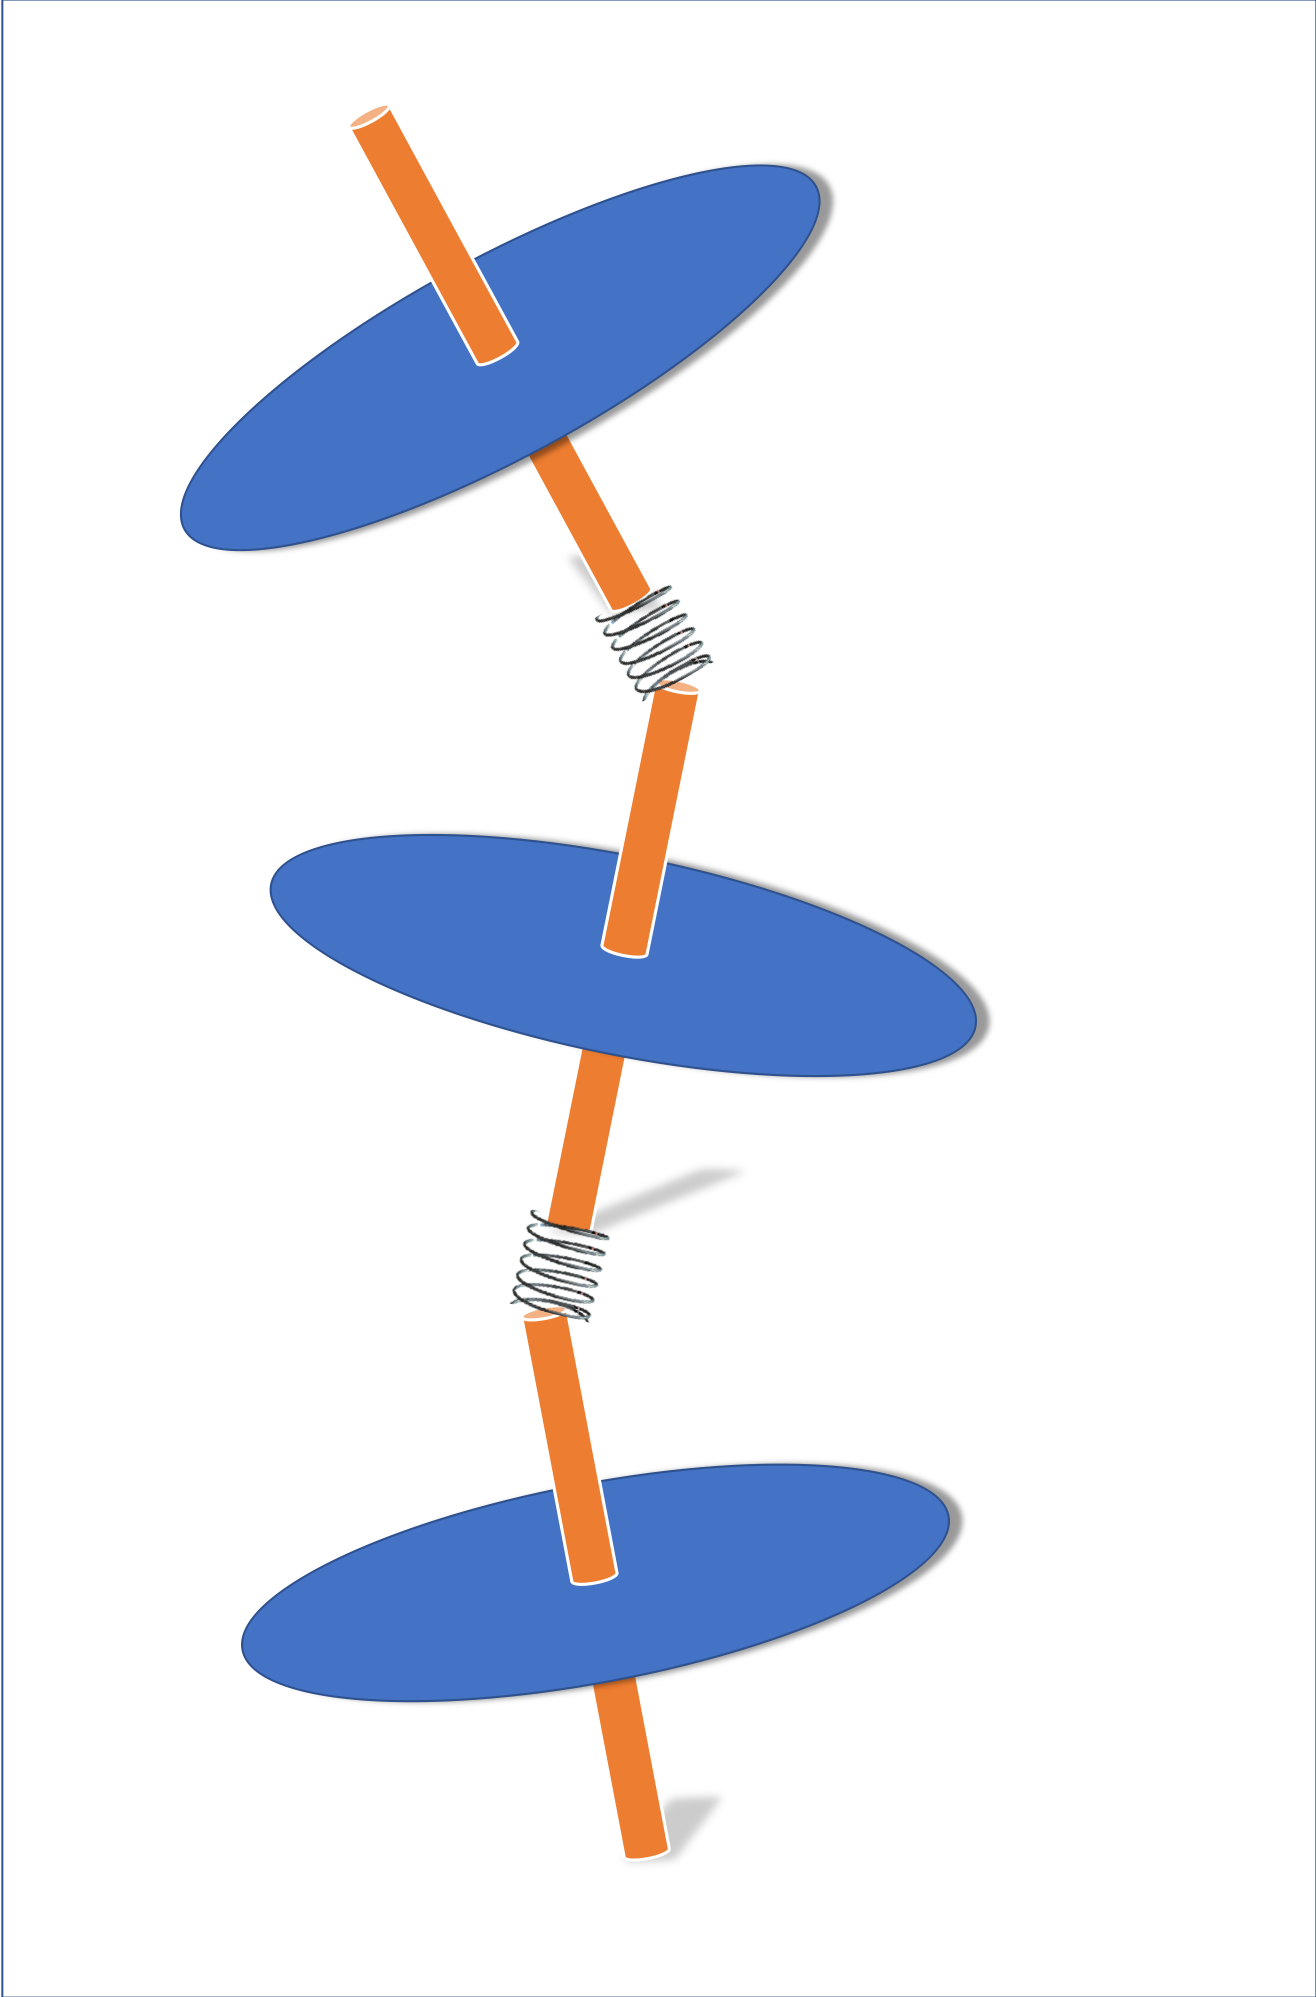
\includegraphics[width=0.4\textwidth, height=8cm]{stack_model.png}
    \caption*{\small Figure 3}
\end {figure}

This model is used to test whether a system consists of more than one gyroscope can maintain a stable periodic motion. In this model, the mass distribution of all gyroscopes are identical and are even. In fact, we set the mass of all nodes to be 1. Results are shown in section 4.2.

\subsection{Gyrocompass}
\hspace{5mm} The basic idea of a gyrocompass is the following: originally a gyroscope is put in a track that is fixed on the horizontal ground (i.e. a tangent plane of the earth's surface). Since the track is fixed, it will move as the earth rotates. We know that a gyroscope has the property of keeping its orientation unchanged, so there will be a relative motion between the gyroscope and its track, thus yielding some dislocation. Consequently, the axis of the gyroscope does not lie on the track any more, instead it may have some elevation. See figure 4.

\begin {figure}[ht]
	\centering
	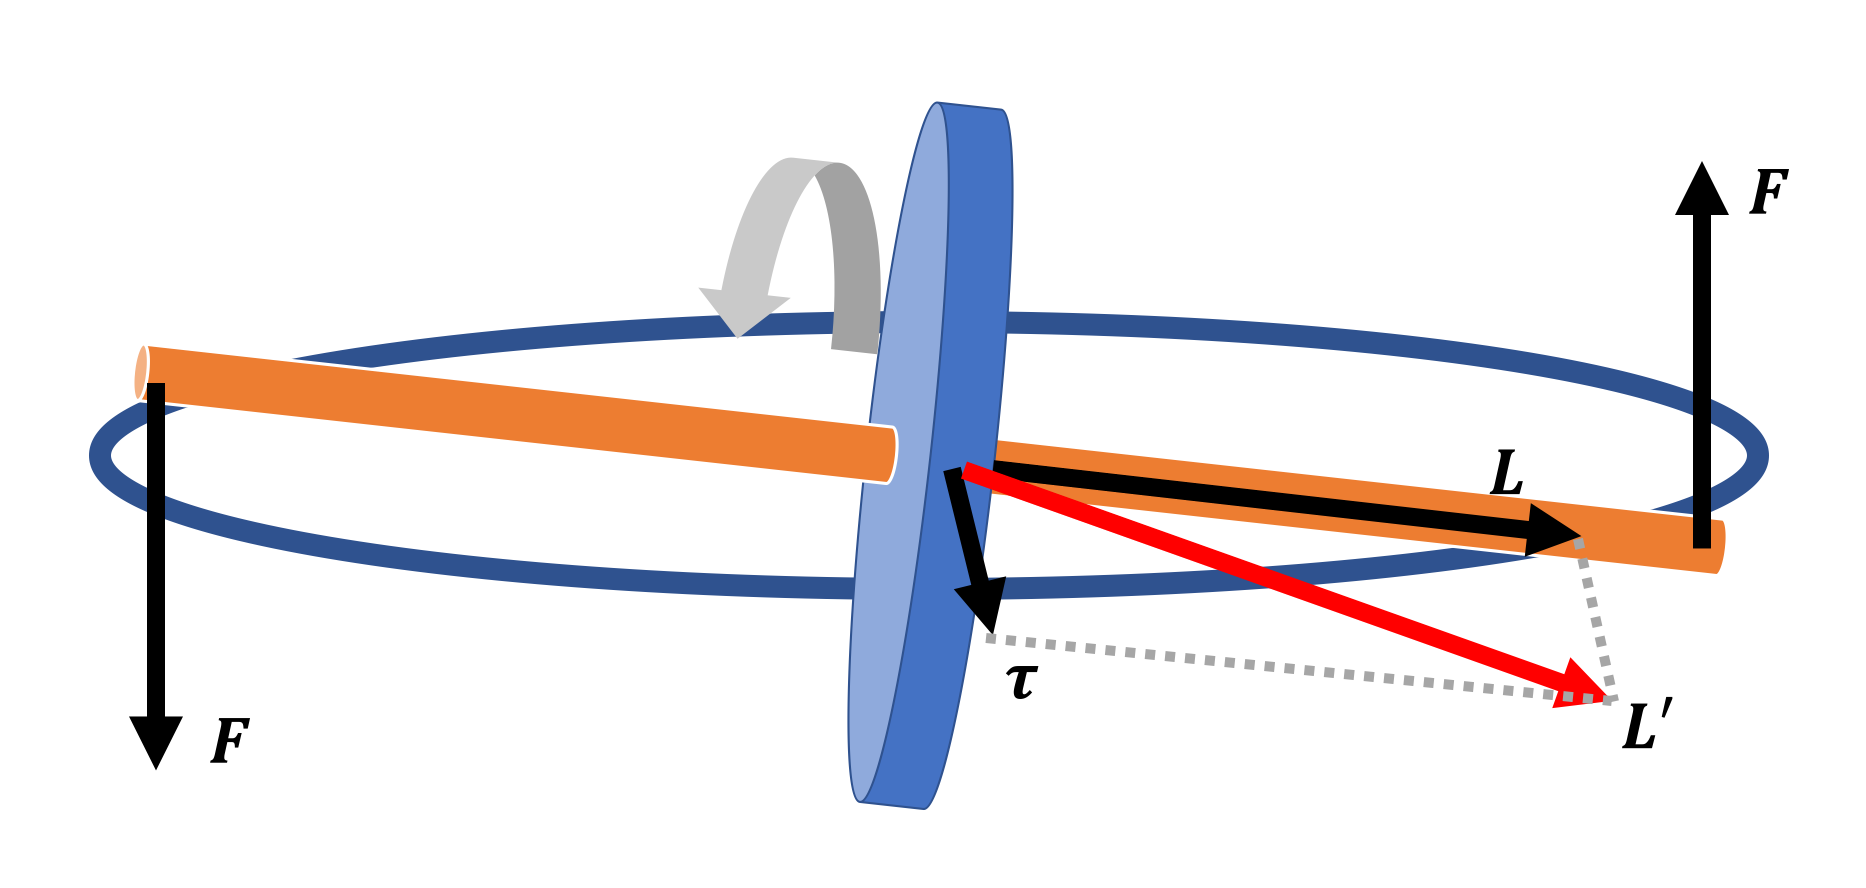
\includegraphics[width=0.6\textwidth]{gyrocompass_physics.png}
	\caption*{\small Figure 4}
	\footnotesize
	\emph{The gyroscope itself is rotating and its angular momentum is given by $\vec{L}.$ When the axis of the gyroscope has some elevation above the track, forces will be applied by the track. The corresponding torque $\vec{\tau}$ and the new angular momentum $\vec{L'}$ (the red arrow) are shown in the graph. }
\end {figure}

Forces are applied on two endpoints of the gyroscope by the track to constrain the axis stay inside the track. Torque $\vec{\tau}$ is generated by the constraining forces, and its direction is on the tangent plane and perpendicular to the current angular momentum $\vec{L}$. As is shown in the graph, the torque will skew the angular momentum from $\vec{L}$ to $\vec{L'}.$ As a result, the axis of gyroscope will start to rotate inside the track. When the earth is rotating, there will be consecutive elevations and hence consecutive constraining forces. This will keep the axis of gyroscope oscillating around the north-south direction. If the track is frictionless, amplitude of oscillation might be large. So it should be ideal that we can add some friction when the axis is rotating in the track, or equivalently, when the two endpoints are gliding in the track.

In real life, another way to build a gyrocompass is to constrain the gyroscope by attaching a pendulum. The idea is the same: we constrain the axis of gyroscope to lie on the tangent plane, but allow it to rotate freely within the plane.

In our model, we simulate a gyrocompass in the following steps. A ball to represent the earth is first constructed. A track is installed at some particular point on the earth. Then a gyroscope is put inside the track, the direction of whose axis should be assigned randomly, since we want to see that the constraining forces can navigate the direction of the axis. This is shown in the figure 5.

\begin{figure}[ht]
	\begin{minipage}{0.33\textwidth}
		\centering
		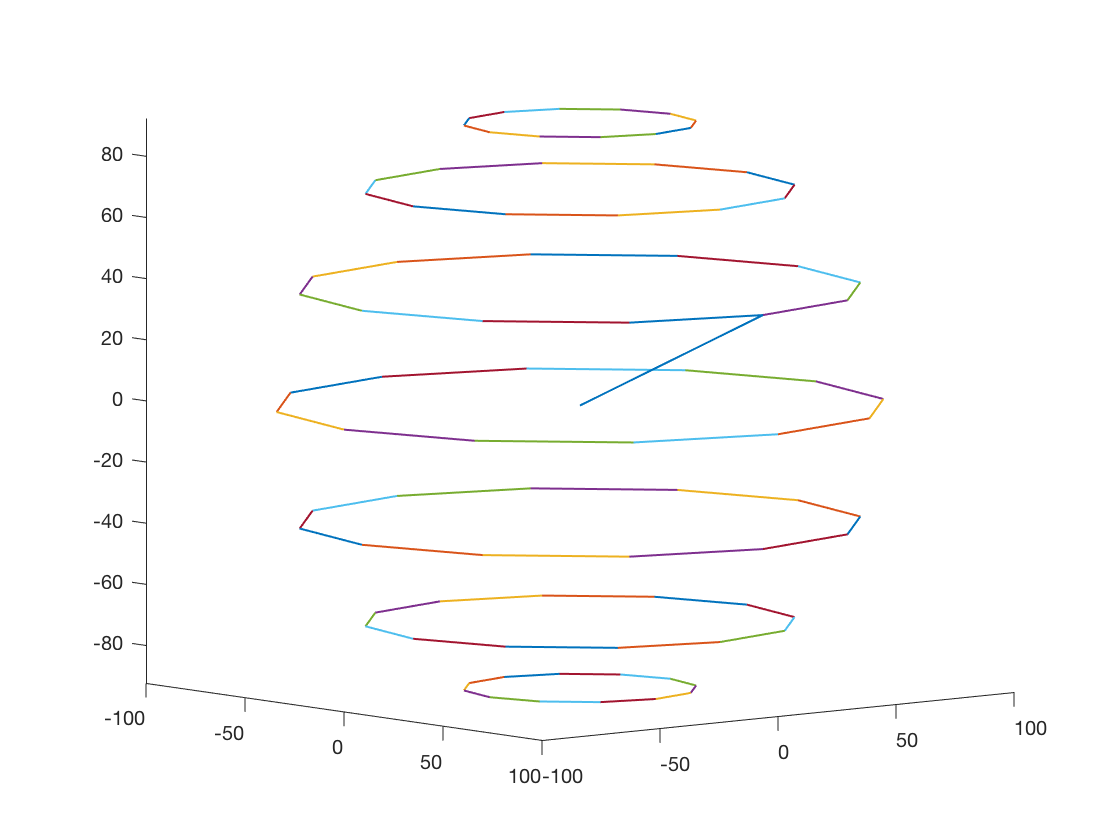
\includegraphics[width=0.99\textwidth]{earth_structure.png}
		\caption*{\small Figure 5(a)}
	\end{minipage}
	\begin{minipage}{0.33\textwidth}
		\centering
		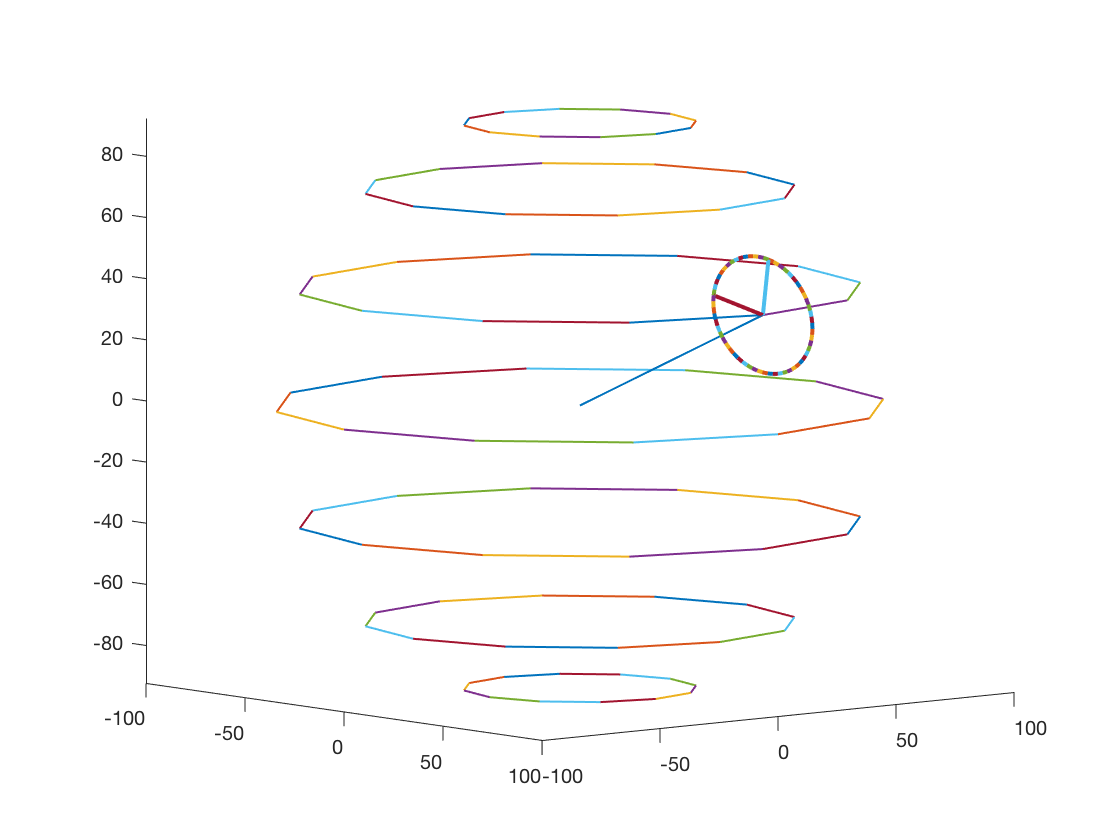
\includegraphics[width=0.99\textwidth]{track_structure.png}
		\caption*{\small Figure 5(b)}
	\end{minipage}
	\begin{minipage}{0.33\textwidth}
		\centering
		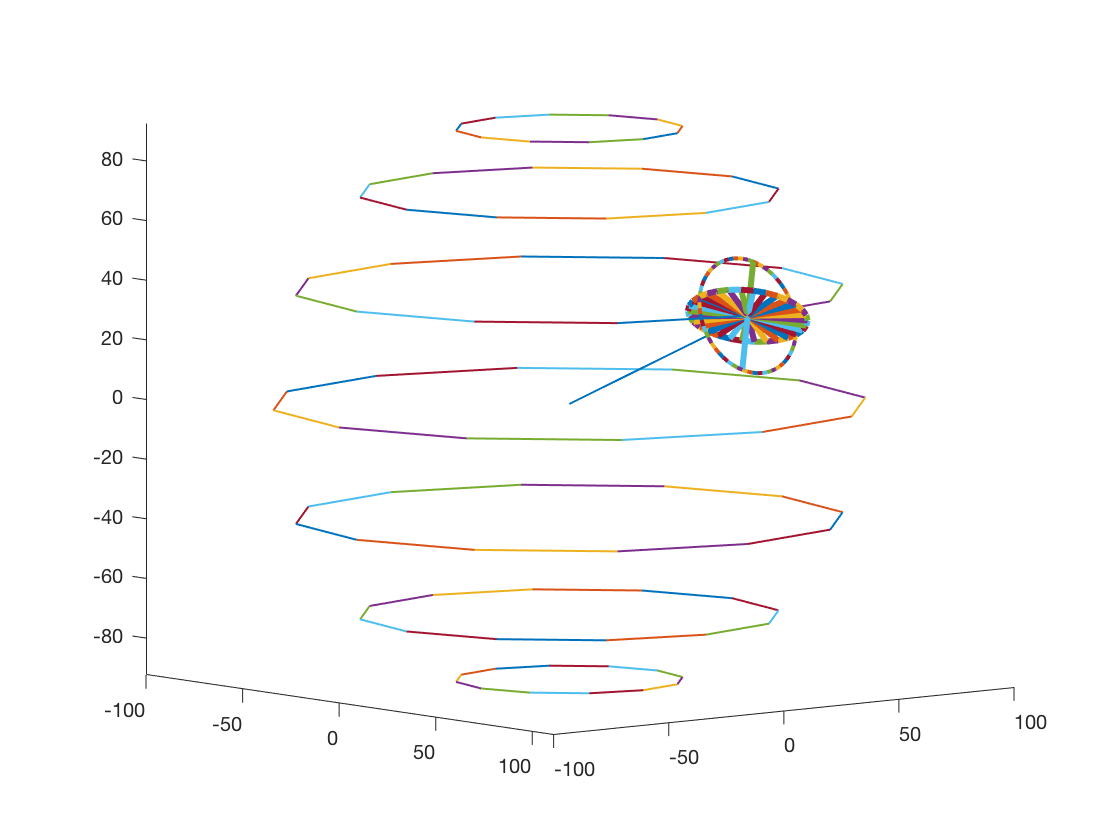
\includegraphics[width=0.99\textwidth]{gyro_structure.png}
		\caption*{\small Figure 5(c)}
	\end{minipage}

	\footnotesize
	\emph{Figure 5(a) is a representation of the earth in which we draw seven latitudes: one equator and three on each hemisphere. A particular radius is drawn. The corresponding point on the surface is the point where we to build the gyrocompass. Figure 5(b) shows that a circular track is assembled on the earth. The complete structure is shown in figure 5(c), where the initial direction of the axis of the gyroscope is arbitrarily assigned.}
\end{figure}

We device that the constraining force acting on each endpoint is proportional to the distance from this endpoint to the track. In other words, if the distance from one endpoint to the tangent plane is positive (i.e. this endpoint is above the plane), a force pointing downward with magnitude proportional to the distance would be exerted on this endpoint. Such a process is repeated at every time step. In addition, in this model we device that the magnitude of friction is proportional to the speed at which the endpoints are gliding, and its direction is opposite to the current velocity. This helps to stabilize the axis so that we can clearly see its oscillation around the north-south direction. For detailed implementation, see the code for this part: \href{https://github.com/zeshunzong/A_series_of_experiments_based_on_gyroscope/blob/master/matlab/gyrocompass_general_demo.m}{\textbf{gyrocompass at northern hemisphere with friction}} and \href{https://github.com/zeshunzong/A_series_of_experiments_based_on_gyroscope/blob/master/matlab/gyrocompass_at_equator.m}{\textbf{gyrocompass at equator without friction}} at \url{https://github.com/zeshunzong/A_series_of_experiments_based_on_gyroscope/blob/master/matlab/gyrocompass_general_demo.m} and \url{https://github.com/zeshunzong/A_series_of_experiments_based_on_gyroscope/blob/master/matlab/gyrocompass_at_equator.m}.

Movies of gyrocompass's motion can be made, and graphs to analyze the axis's oscillation can be drawn. See the next section.



\section{Results}
\subsection{A Simple Gyroscope}
\hspace{5mm} Our model successfully simulates the motion of gyroscopes with different mass distributions. In our model, the normal force and friction is large enough so that the movement of the bottom node on the axis is negligible. Therefore, we use the trace of the top node to describe the motion of a simple system that consists of only one gyroscope. We first examine the effect of a rotation of the starting position on the trace of the system. We proceed by recording the trace of a particular mass distribution, then rotating the starting position of the gyroscope while keeping all other parameters the same and at last recording the new trace. Figure 6 shows the trace of two different mass distributions and their rotations. In both cases, the three nodes on the axis have mass 1 (gravity coefficient is 10). The radius of the wheel is 1 and length of the axis is 1.8. And the starting angular momentum points in the direction $[\sin(\pi/12), 0, \cos(\pi/12)]$.

\begin{figure}[ht]
	\begin{minipage}{0.5\textwidth}
		\centering
		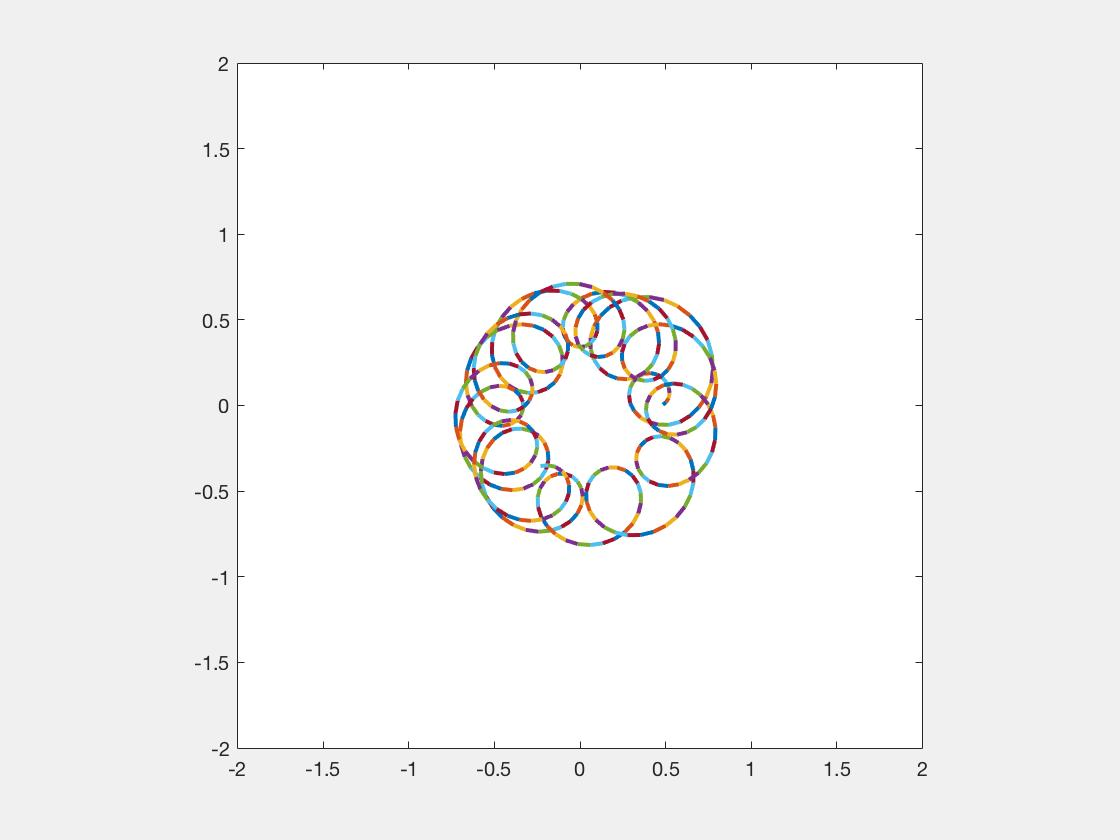
\includegraphics[width=0.89\textwidth]{uneven_firsthalf.jpg}
		\caption*{\small Figure 6(a)}
	\end{minipage}
	\begin{minipage}{0.5\textwidth}
		\centering
		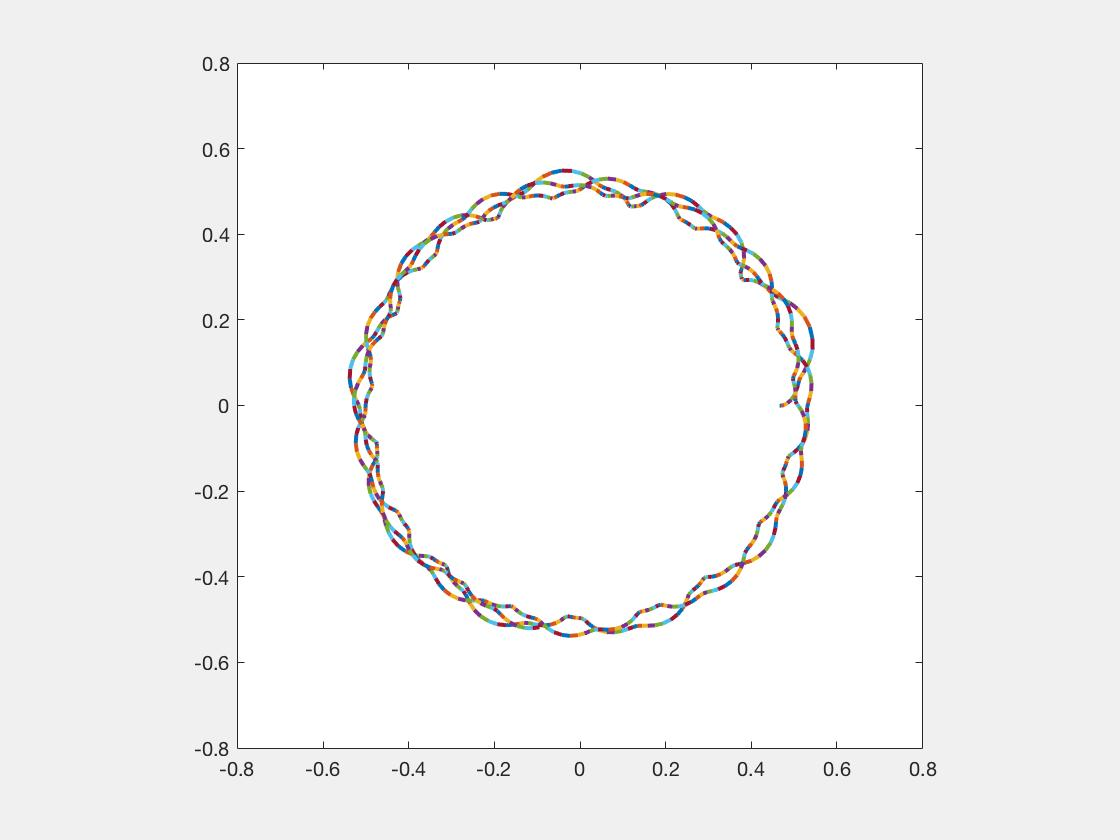
\includegraphics[width=0.89\textwidth]{uneven_trisection_L150.jpg}
		\caption*{\small Figure 6(c)}
	\end{minipage}
	\begin{minipage}{0.5\textwidth}
		\centering
		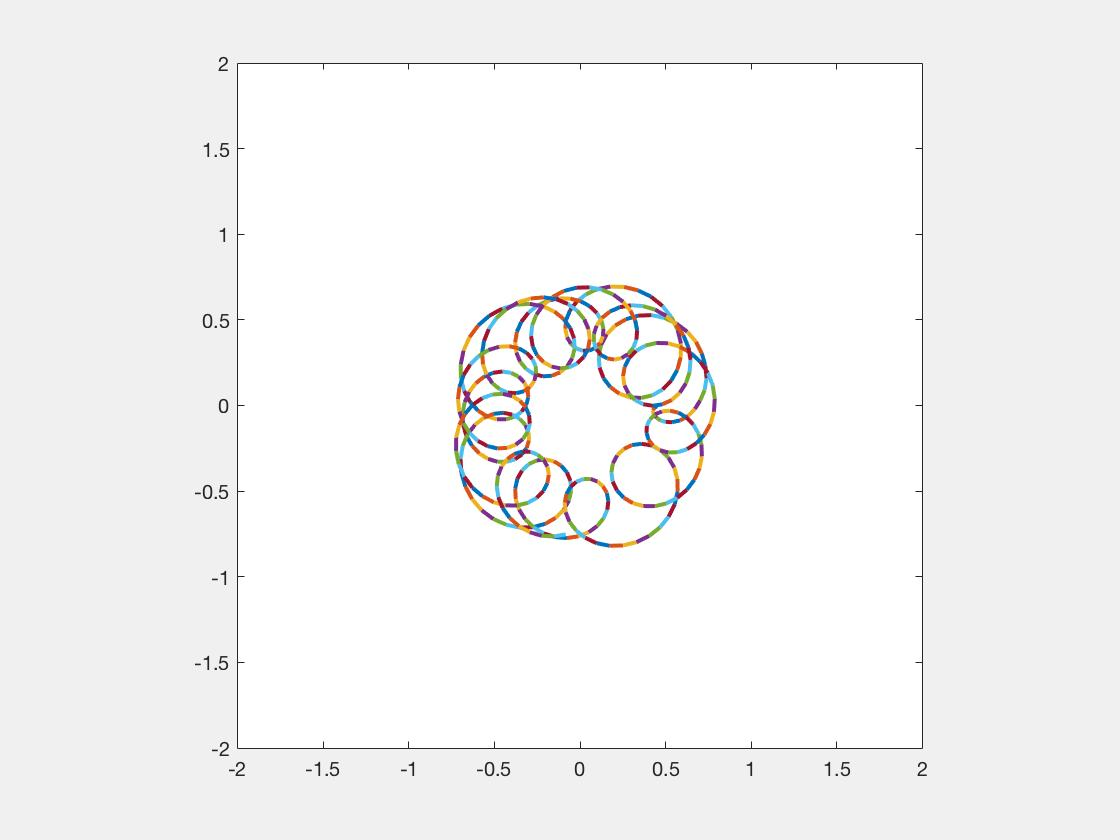
\includegraphics[width=0.89\textwidth]{uneven_secondhalf.jpg}
		\caption*{\small Figure 6(b)}
	\end{minipage}
	\begin{minipage}{0.5\textwidth}
		\centering
		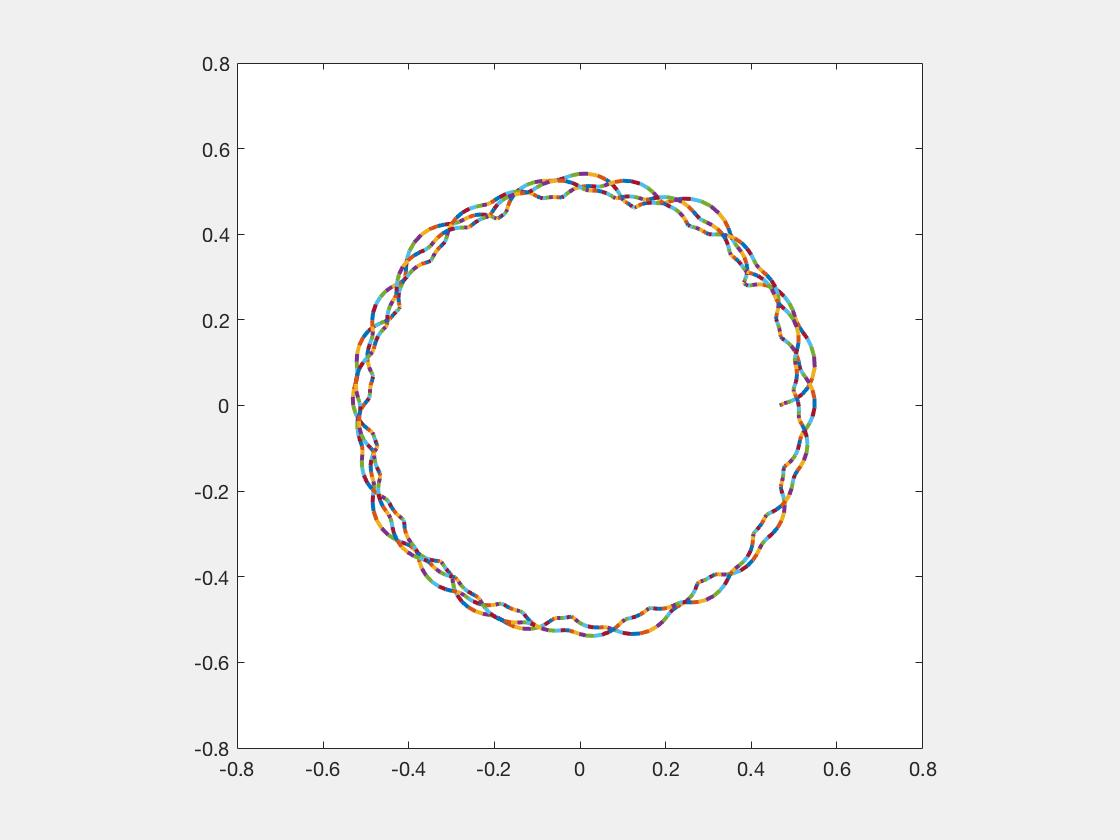
\includegraphics[width=0.89\textwidth]{uneven_trisection_rotation.jpg}
		\caption*{\small Figure 6(d)}
	\end{minipage}
\end{figure}

\begin{figure} [ht]
    \centering
    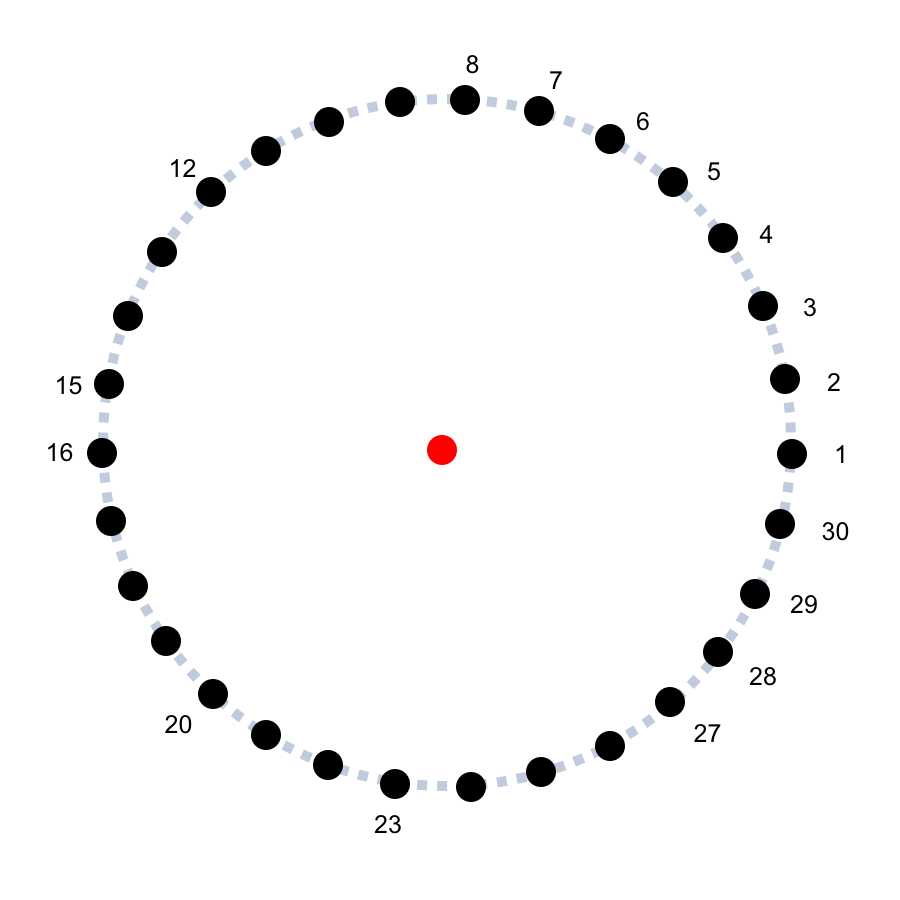
\includegraphics[width=0.3\textwidth]{masses_demo.png}
    \caption*{Figure 7: Wheel of the gyroscope}
    \label{fig:my_label}
\end{figure}

\vspace{\baselineskip}
In our first distribution, nodes 1-15 have mass 1 and nodes 16-30 have mass 0.8. The magnitude of the starting angular momentum is 300. The result is presented in Figure 6(a). A 180-degree rotation gives us a mass distribution of nodes 1-15 with mass 0.8 and nodes 16-30 with mass 1. The result is shown in Figure 6(b). In our second distribution, nodes 1-5, 16-20 have mass 1 and all other nodes on the wheel have mass 0. The magnitude of the starting angular momentum is 300. The result is shown in Figure 6(c). Figure 6(d) is the trace of a system with nodes 8-12, 23-27 having mass 1 and all other nodes on the wheel have mass 0 (a rotation of the mass distribution in 6(c)). In both cases, it is obvious that a rotation of the original mass distribution produces a very similar trace. Our model suggests that a rotation of the mass distribution does not change the behavior of the gyroscope much.

This model also shows a relation between the angular momentum of the system and its trace. The following three diagrams are the traces of a gyroscope with even mass distribution (all nodes have mass 1). Note that the angular momentum starts in the same direction. Therefore the only thing different in the three tests is the magnitude of the starting angular momentum.
\begin{figure}[ht]
	\begin{minipage}{0.33\textwidth}
		\centering
		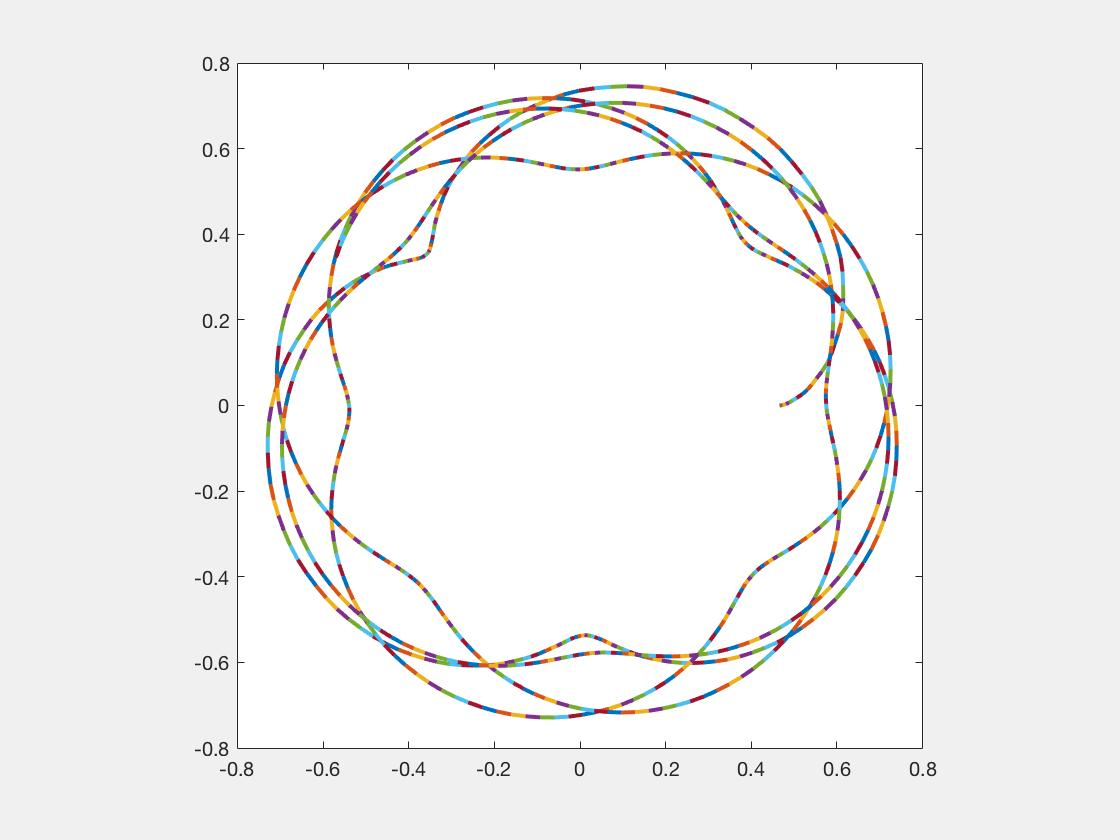
\includegraphics[width=0.89\textwidth]{even_L270.jpg}
		\caption*{\small Figure 8(a), $\parallel$ L $\parallel$ = 270}
	\end{minipage}
	\begin{minipage}{0.33\textwidth}
		\centering
		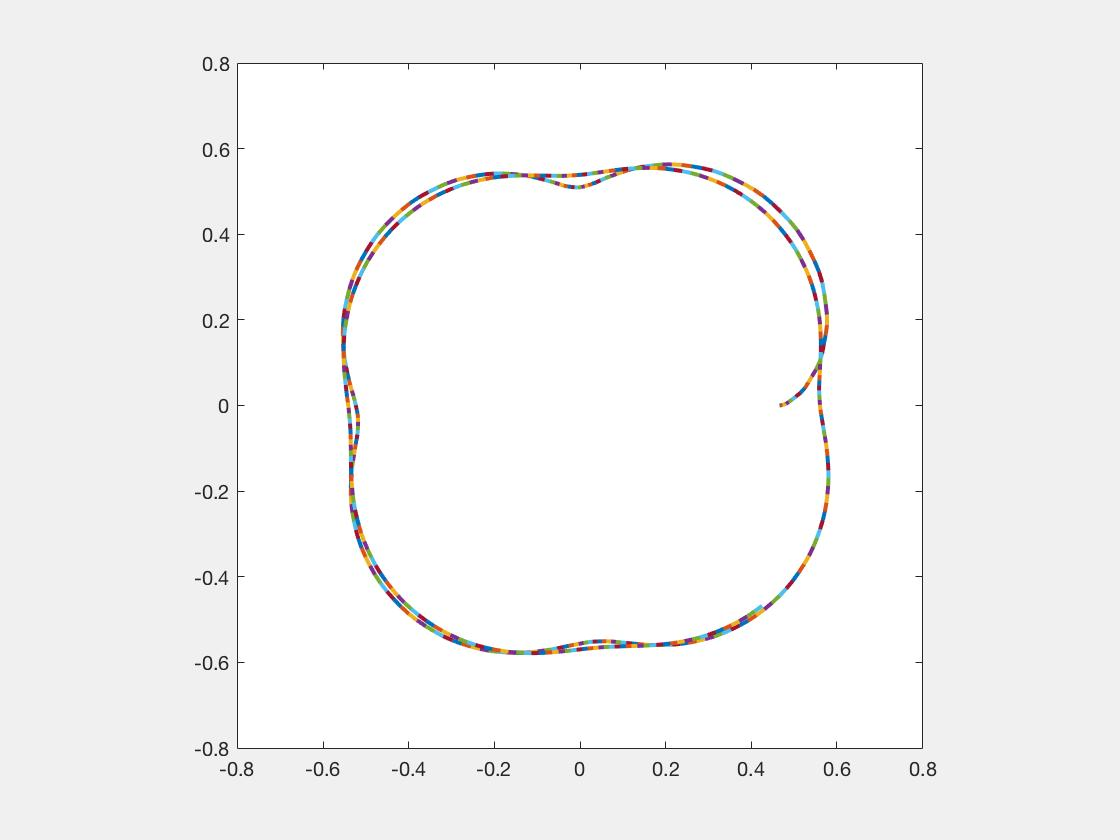
\includegraphics[width=0.89\textwidth]{even_L300.jpg}
		\caption*{\small Figure 8(b), $\parallel$ L $\parallel$ = 300}
	\end{minipage}
	\begin{minipage}{0.33\textwidth}
		\centering
		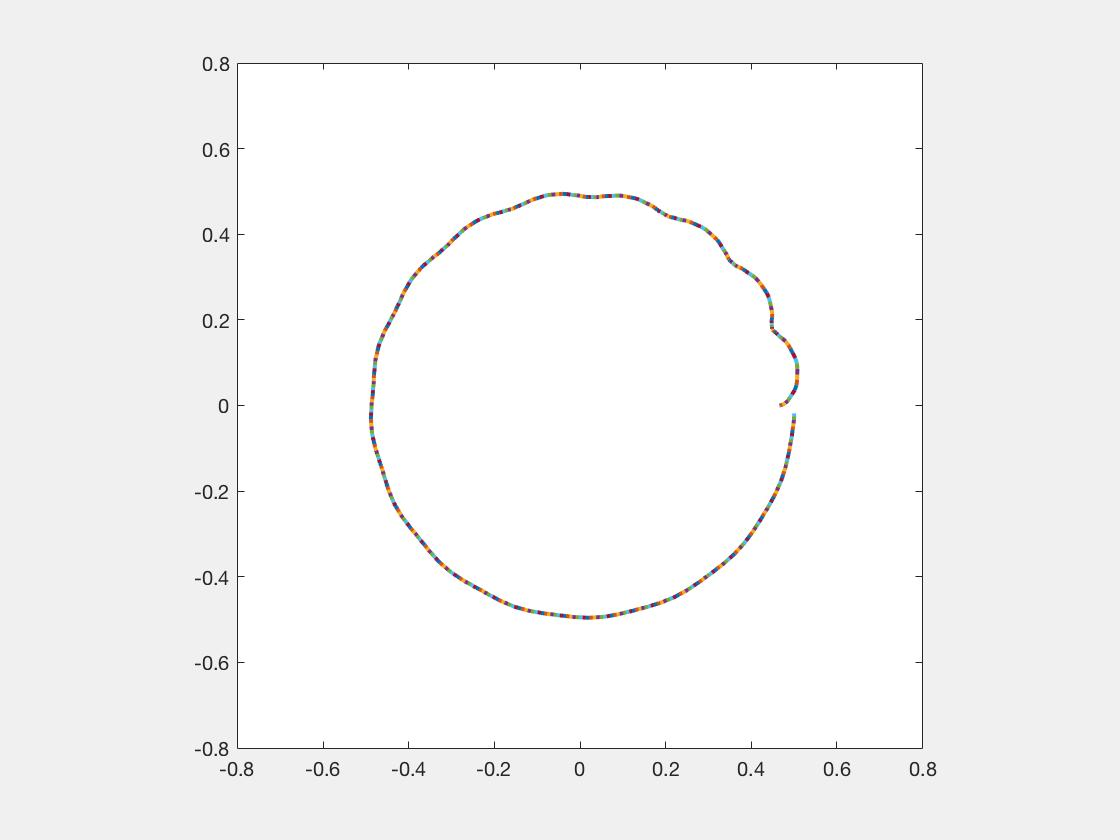
\includegraphics[width=0.89\textwidth]{even_L500.jpg}
		\caption*{\small Figure 8(c), $\parallel$ L $\parallel$ = 500}
	\end{minipage}
\end{figure}

As demonstrated in this example, the gyroscope doesn't move in a perfectly circular motion. However, the larger angular momentum is, the more circular the trace is. The result holds for other mass distributions. We will use the second uneven mass distributions we used before as an example.
\begin{figure}[ht]
	\begin{minipage}{0.33\textwidth}
		\centering
		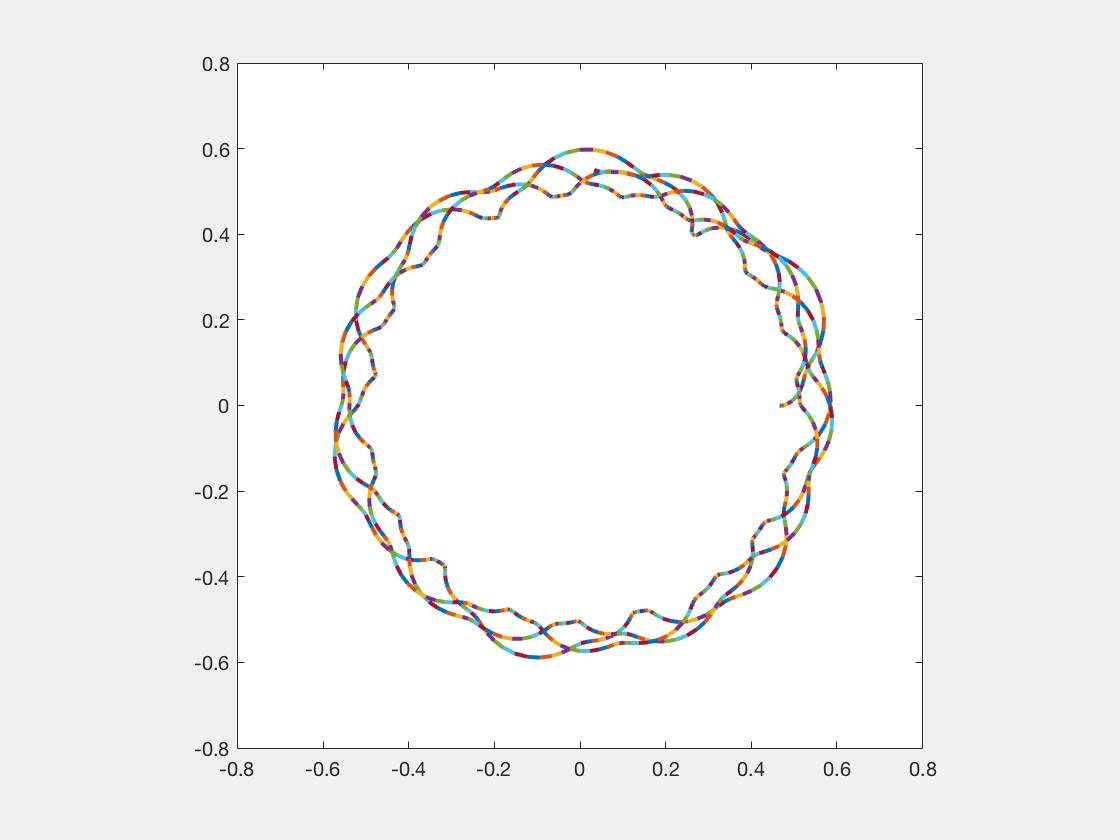
\includegraphics[width=0.89\textwidth]{uneven_trisection_L130.jpg}
		\caption*{\small Figure 9(a), $\parallel$ L $\parallel$ = 130}
	\end{minipage}
	\begin{minipage}{0.33\textwidth}
		\centering
		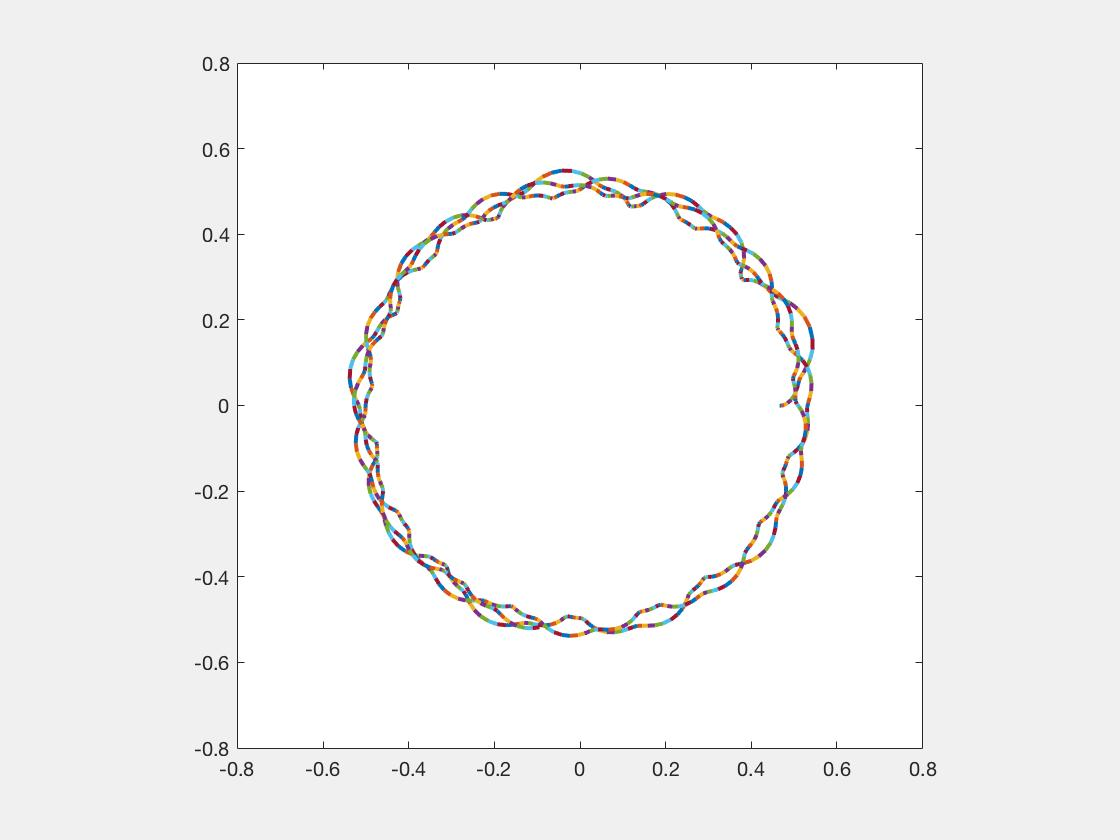
\includegraphics[width=0.89\textwidth]{uneven_trisection_L150.jpg}
		\caption*{\small Figure 9(b), $\parallel$ L $\parallel$ = 150}
	\end{minipage}
	\begin{minipage}{0.33\textwidth}
		\centering
		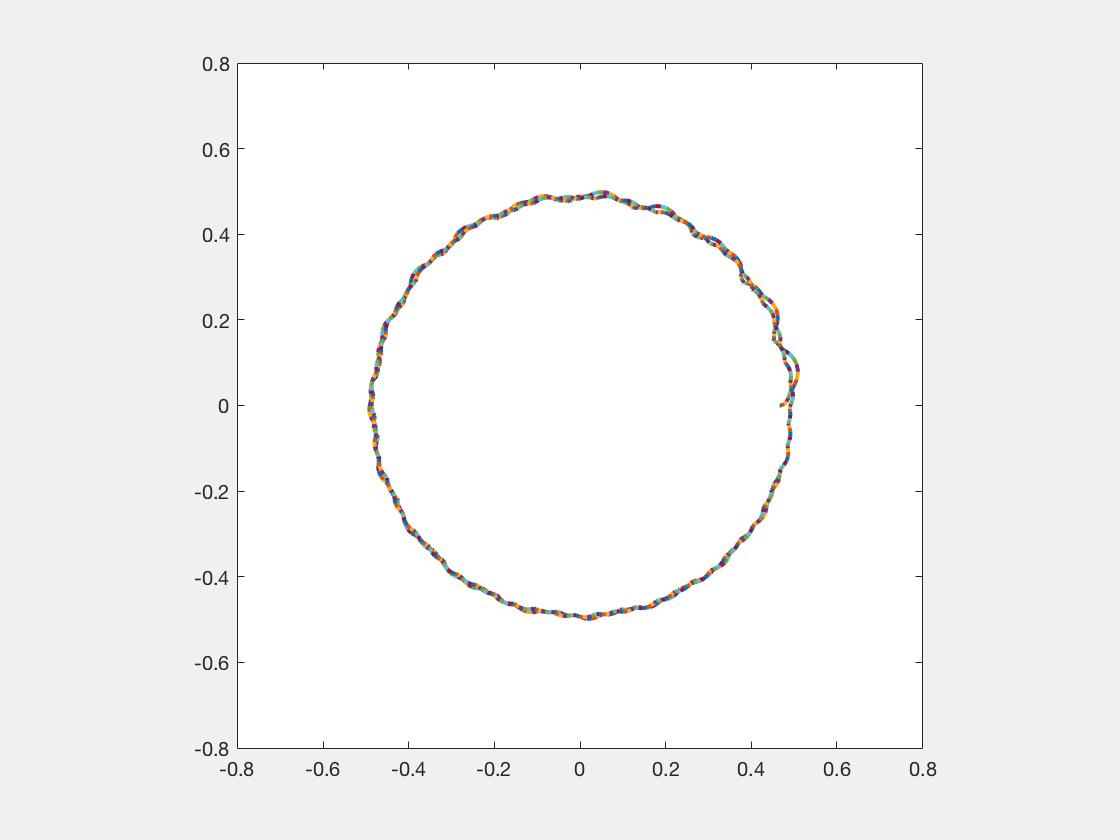
\includegraphics[width=0.89\textwidth]{uneven_trisection_L200.jpg}
		\caption*{\small Figure 9(c), $\parallel$ L $\parallel$ = 200}
	\end{minipage}
\end{figure}

Note that the \text{``}circleness\text{''} of the trace is actually determined by its angular velocity. In the algorithm we presented in section 4.1, $\widetilde{X}$ depends only on angular velocity $\omega$. But in the above two examples, we fixed the mass distribution and thus fixing the moment of inertia. As a result, $\Omega = I^{-1}L$ is proportional to $L$. The result is quite intuitive.

\subsection{Stack of Gyroscopes}
\hspace{5mm} In this system, we only consider gyroscopes with a uniform mass distribution (all nodes have mass 1). Although we did model systems with three gyroscopes, they are very unstable and there are too many parameters involved. (an example is presented here: \url{https://github.com/zeshunzong/A_series_of_experiments_based_on_gyroscope/tree/master/video/stacked_gyro}) Therefore, we only concern ourselves with two gyroscopes here. We first tilt the bottom gyroscope so that the axis of ratation points towards $[\sin(\pi/12), 0, \cos(\pi/12)]$. We then tilt  the upper gyroscope back so that it points vertically upward. Both gyroscopes have an starting angular momentum that points in the same direction as the axis of rotation and have magnitude 600. Here's a video that shows its motion: \url{https://github.com/zeshunzong/A_series_of_experiments_based_on_gyroscope/tree/master/video/stacked_gyro/two_stack.mov}

In this model, we wanted to observe the relationship between the stability of the system and the direction of the spin. We changed the direction of the angular momentum of the second gyroscope to $[-\sin(\pi/12), 0, -\cos(\pi/12)]$ (180 degree turn) while keeping all other parameters the same. The behavior of the resulting system seems slightly more unstable. The video can be watched here: \url{https://github.com/zeshunzong/A_series_of_experiments_based_on_gyroscope/tree/master/video/stacked_gyro/two_stack_backwards.mov}


\subsection{Gyrocompass}
\hspace{5mm} Our model successfully simulated the process that a gyroscope, with its axis fixed on a tangent plane, starting at any random orientation, could navigate itself so that its axis would oscillate around the north-south direction. Noticeably, we can see that, after the gyroscope settles down, both the gyroscope and the earth are rotating eastward (or, from west to east). This gives us a way, in real life, to tell which direction that the gyrocompass points is north. We have chosen some point on the northern hemisphere and assemble our gyrocompass there. Two movies shown how it works can be watched at \url{https://github.com/zeshunzong/A_series_of_experiments_based_on_gyroscope/blob/master/video/gyrocompass_at_equator/gyro_wfriction_autoview.mov} and \url{https://github.com/zeshunzong/A_series_of_experiments_based_on_gyroscope/blob/master/video/gyrocompass_at_equator/gyro_wfriction_fixedview.mov}. A snapshot of the gyrocompass is shown in Figure 10. Also, by adding friction, we have managed to decrease the amplitude of oscillation.

\begin{figure}[ht]
	\centering
	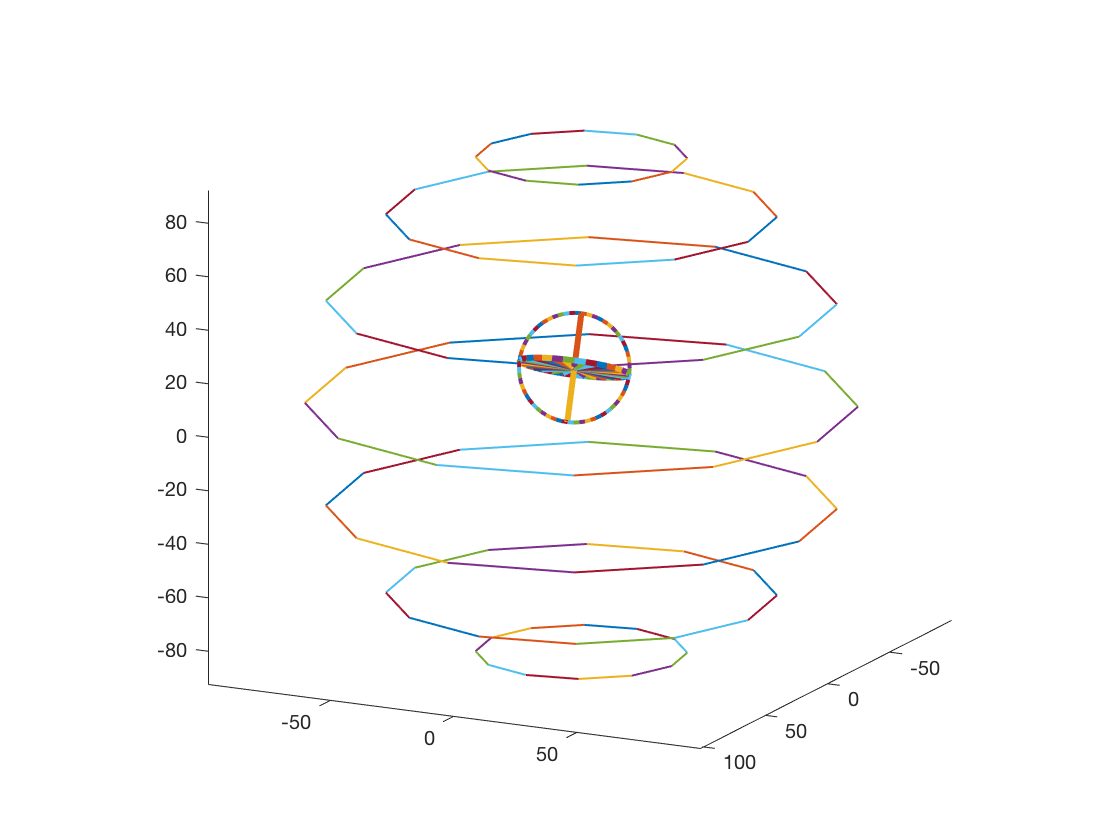
\includegraphics[width=0.5\textwidth]{demo_pointing_north.png}		\caption*{\small Figure 10}
	\footnotesize
	\emph{This figure is a snapshot of gyrocompass put at a point on the northern hemisphere. Observe that its axis is pointing roughly to the north. In the movie we can see that its axis is actually oscillating around the north, with an amplitude of about 25 degrees. Note that friction is exerted when the axis is gliding on the track. In this way we can decrease the magnitude of oscillation.}
\end{figure}

Next we consider a gyrocompass put at the equator and analyze the oscillation of its axis. Initially the axis of the gyroscope is set to point eastward. This setup is shown in figure 11. We define $\phi$ to be the angle between the gyroscope's axis and the vector pointing eastward, so if the gyrocompass is pointing north, $\phi = \frac{\pi}{2}.$ See figure 12. A movie shown its oscillation can be found \href{https://github.com/zeshunzong/A_series_of_experiments_based_on_gyroscope/blob/master/video/gyrocompass_at_equator/gyro_EQ_init_E.mov}{\textbf{here}} at \url{https://github.com/zeshunzong/A_series_of_experiments_based_on_gyroscope/blob/master/video/gyrocompass_at_equator/gyro_EQ_init_E.mov}. Notice that here no friction is added, so the amplitude of oscillation is 90 degrees. It is expected that the period of oscillation is related to the angular velocities of both the earth and the gyroscope. By plotting the change of angle $\phi$ with respect to time at different combinations of angular velocities, we have confirmed that the faster either rotation is, the shorter the oscillating period would be.
\begin{figure}[ht]
	\begin{minipage}{0.5\textwidth}
		\centering
		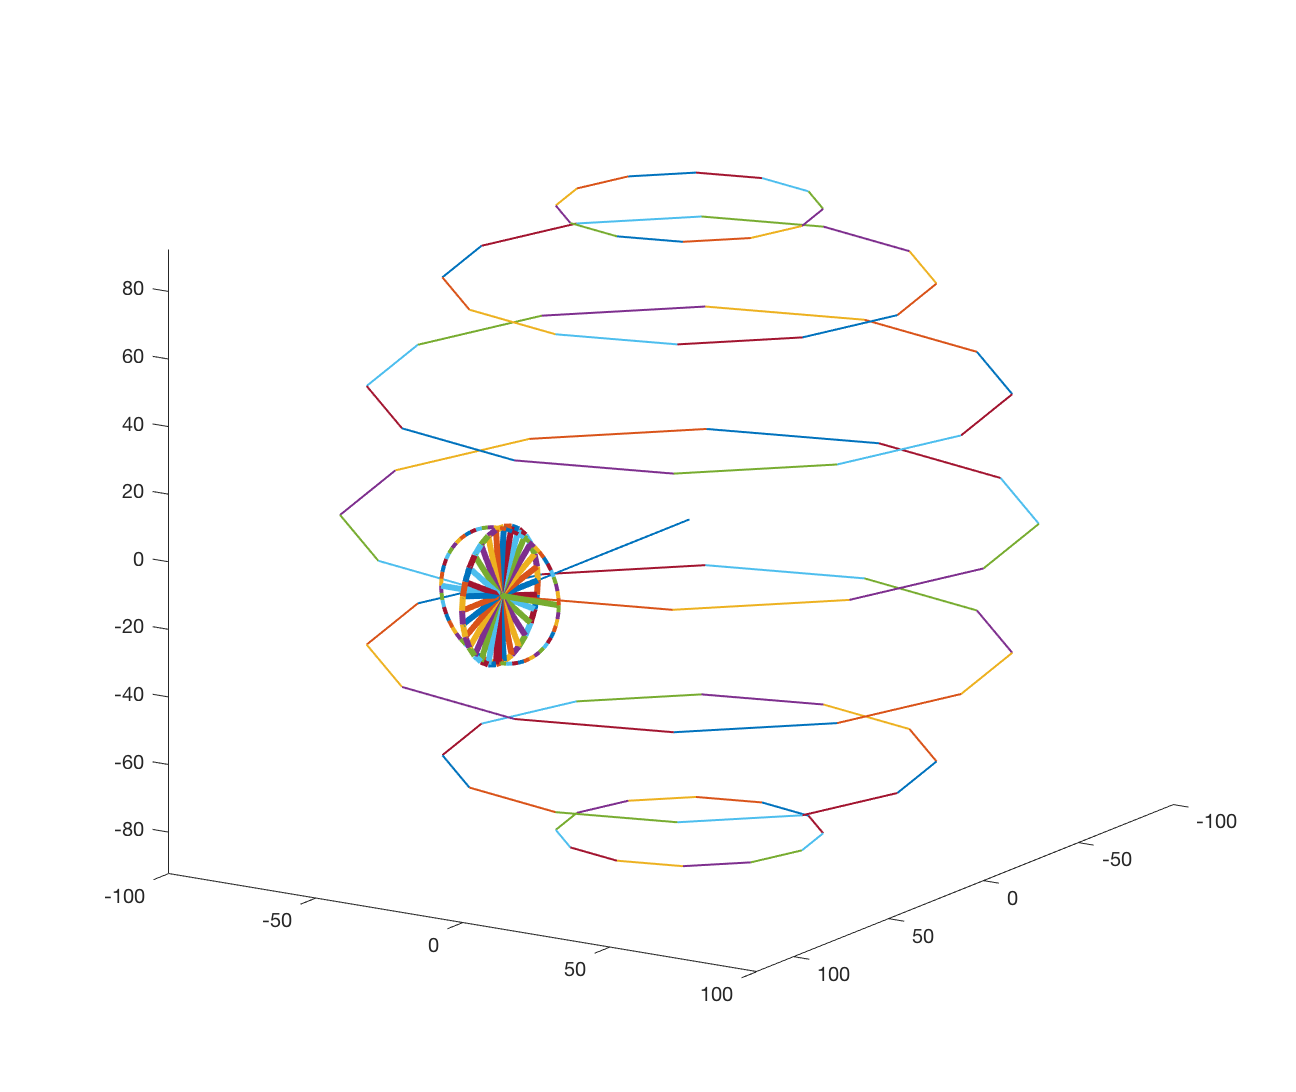
\includegraphics[width=0.7\textwidth]{gyrocompass_at_equator.png}
		\caption*{\small Figure 11}
	\end{minipage}
	\begin{minipage}{0.5\textwidth}
		\centering
		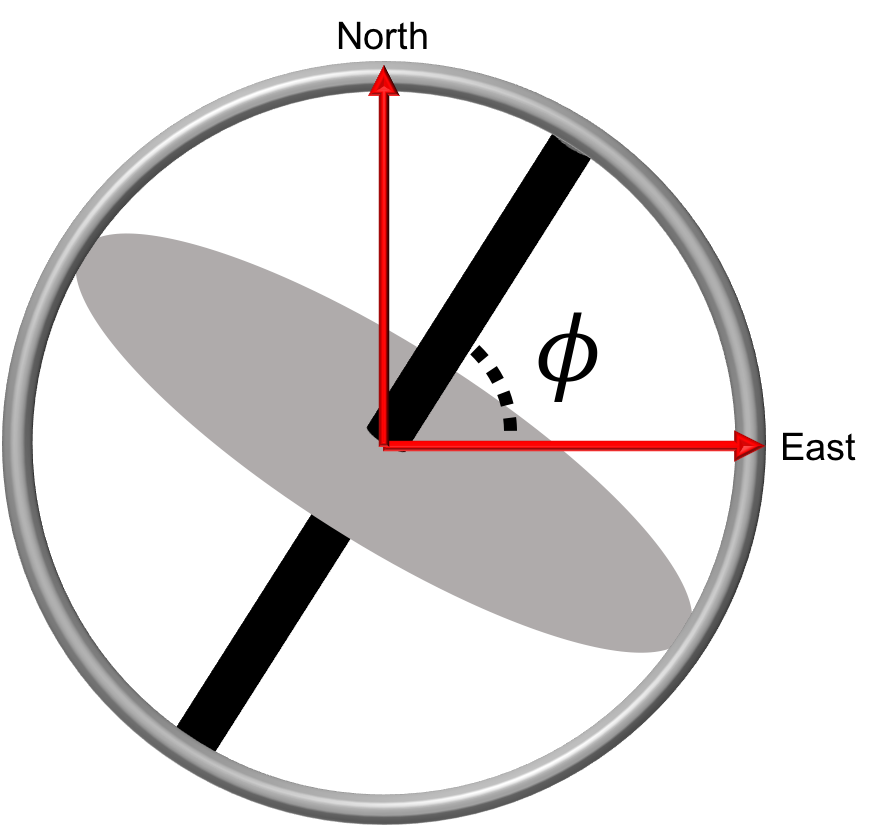
\includegraphics[width=0.55\textwidth]{define_phi.png}
		\caption*{\small Figure 12}
	\end{minipage}
\end{figure}



In fact, quantitative relation between oscillating period of the axis and the two angular velocities can also be established. Figure 13 shows the value of $\phi$ with respect to time. In the first row, the angular velocity of the earth is fixed at some $\vec{\Omega_0},$ while the angular velocity of the gyrocompass is set to be $\frac{1}{2}\vec{\omega_0}$, $\vec{\omega_0},$ and $2\vec{\omega_0}$ respectively. In the second row, the angular velocity of the gyroscope is fixed at $\vec{\omega_0},$ while the angular velocity of the earth is set to be $\frac{1}{2}\vec{\Omega_0}$, $\vec{\Omega_0},$ and $2\vec{\Omega_0}$ respectively. For numerical values of such angular velocities and unit of measure of time (horizontal axis), see the corresponding code \href{https://github.com/zeshunzong/A_series_of_experiments_based_on_gyroscope/blob/master/matlab/gyrocompass_at_equator.m}{\textbf{gyrocompass at equator}} at \url{https://github.com/zeshunzong/A_series_of_experiments_based_on_gyroscope/blob/master/matlab/gyrocompass_at_equator.m}.

\begin{figure}[h]
	\begin{minipage}{0.33\textwidth}
		\centering
		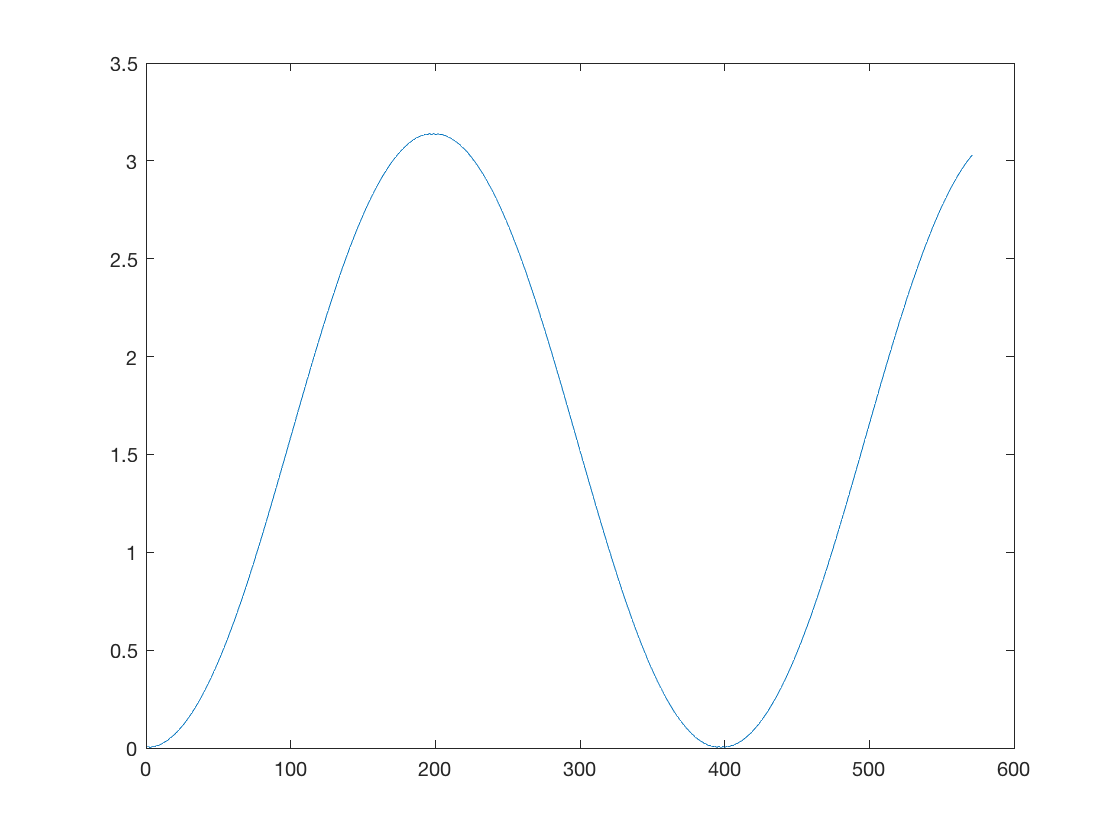
\includegraphics[width=0.89\textwidth]{L5000.png}
		\caption*{\small Figure 13(a), $\vec{\omega} = \frac{1}{2}\vec{\omega_0}, \vec{\Omega} = \vec{\Omega_0}$}
	\end{minipage}
	\begin{minipage}{0.33\textwidth}
		\centering
		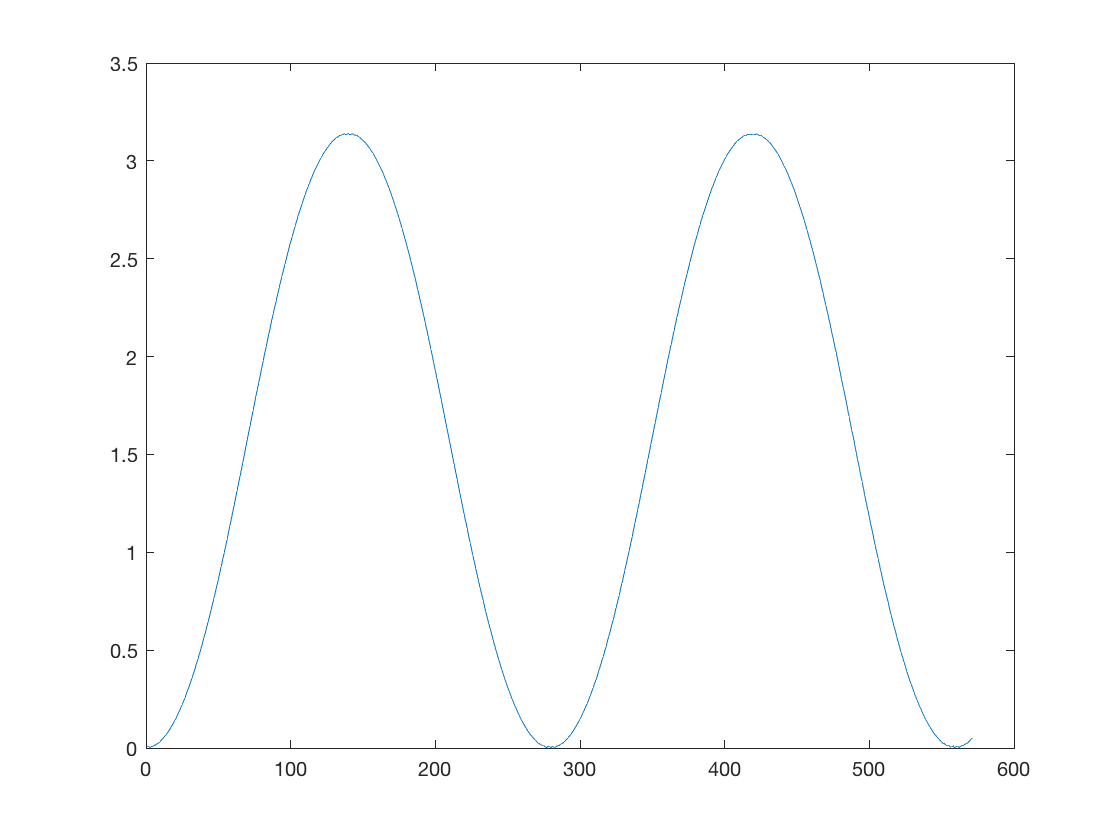
\includegraphics[width=0.89\textwidth]{L10000.png}
		\caption*{\small Figure 13(b), $\vec{\omega} = \vec{\omega_0}, \vec{\Omega} = \vec{\Omega_0}$}
	\end{minipage}
	\begin{minipage}{0.33\textwidth}
		\centering
		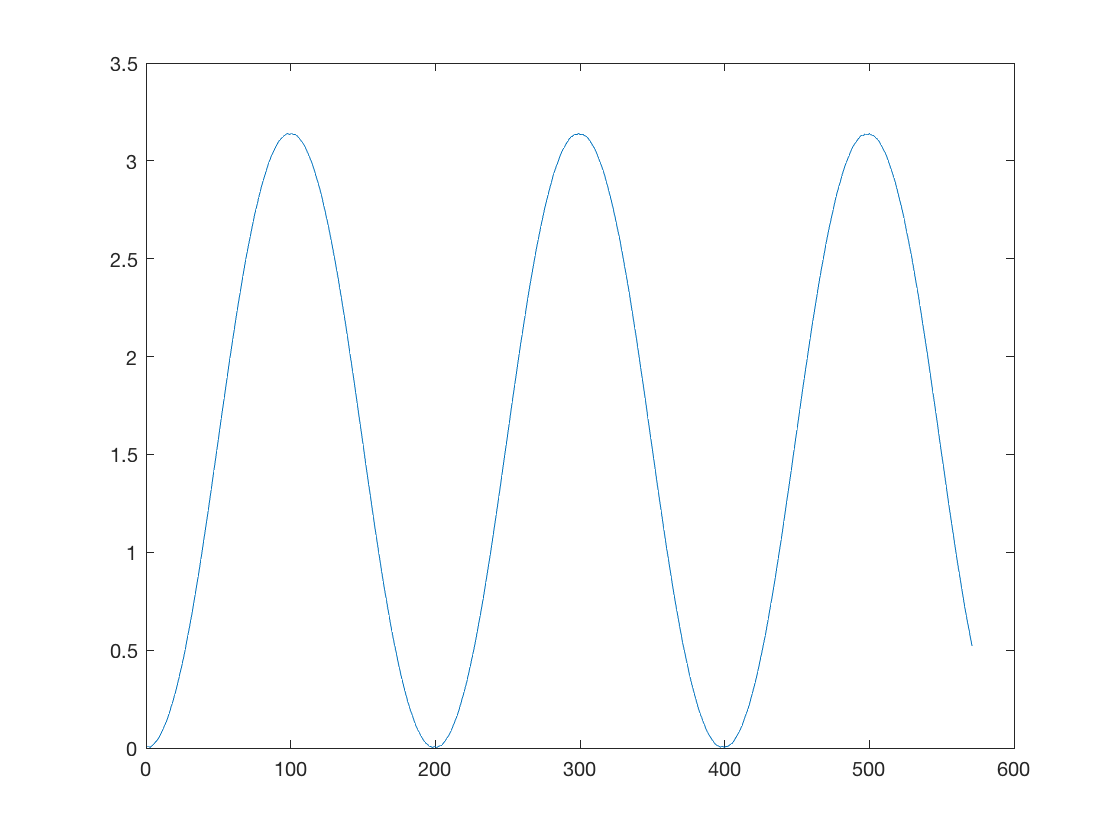
\includegraphics[width=0.89\textwidth]{L20000.png}
		\caption*{\small Figure 13(c), $\vec{\omega} = 2\vec{\omega_0}, \vec{\Omega} = \vec{\Omega_0}$}
	\end{minipage}
	\begin{minipage}{0.33\textwidth}
		\centering
		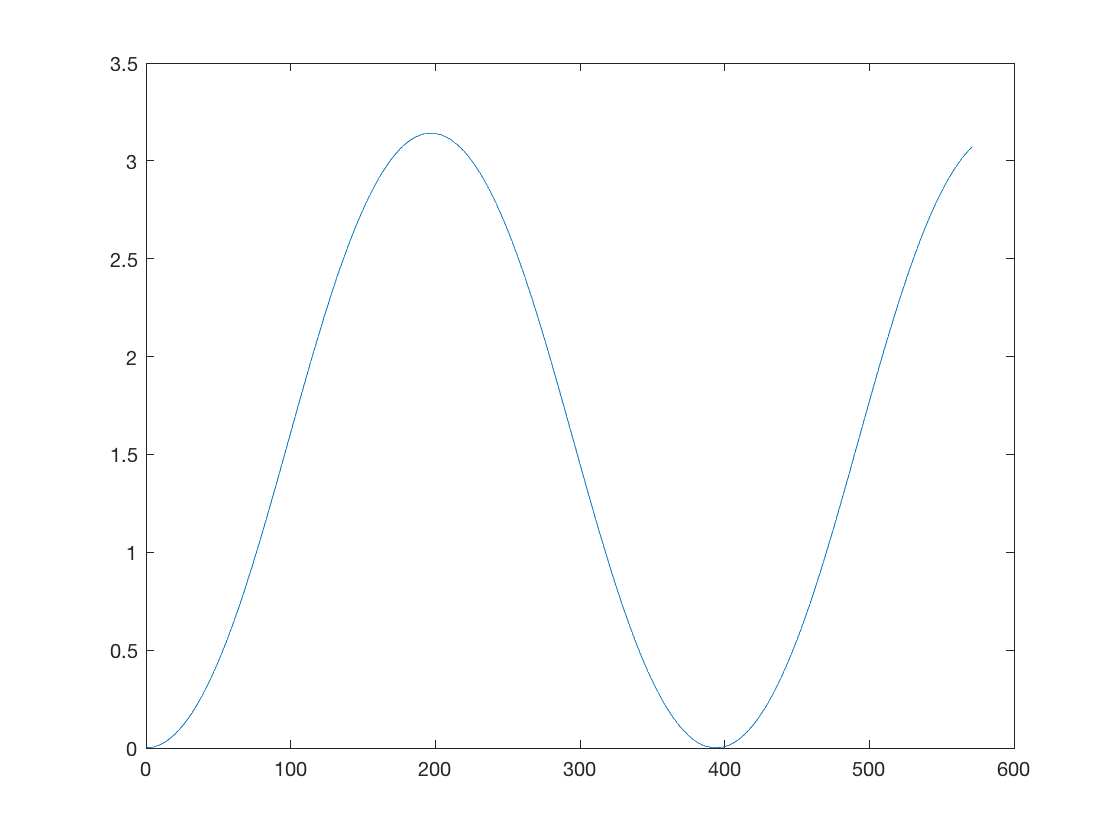
\includegraphics[width=0.89\textwidth]{E500.png}
		\caption*{\small Figure 13(d), $\vec{\omega} = \vec{\omega_0}, \vec{\Omega} = \frac{1}{2}\vec{\Omega_0}$}
	\end{minipage}
	\begin{minipage}{0.33\textwidth}
		\centering
		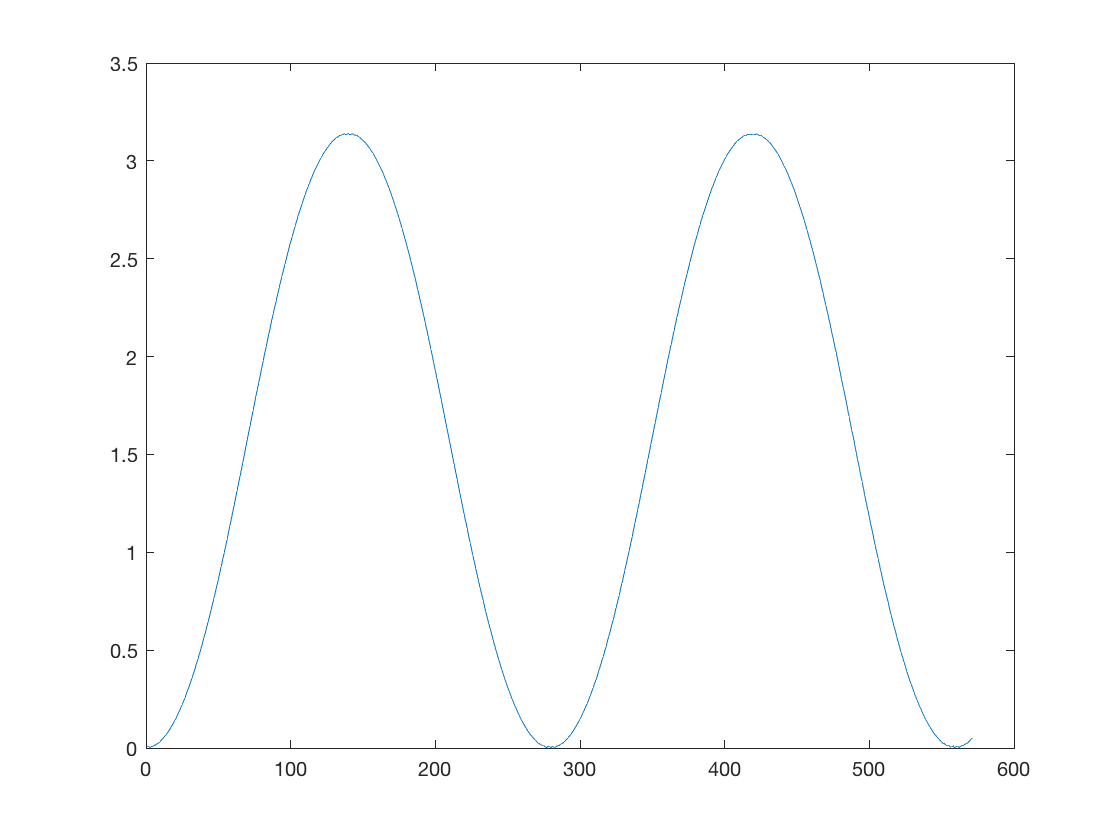
\includegraphics[width=0.89\textwidth]{E1000.png}
		\caption*{\small Figure 13(e), $\vec{\omega} = \vec{\omega_0}, \vec{\Omega} = \vec{\Omega_0}$}
	\end{minipage}
	\begin{minipage}{0.33\textwidth}
		\centering
		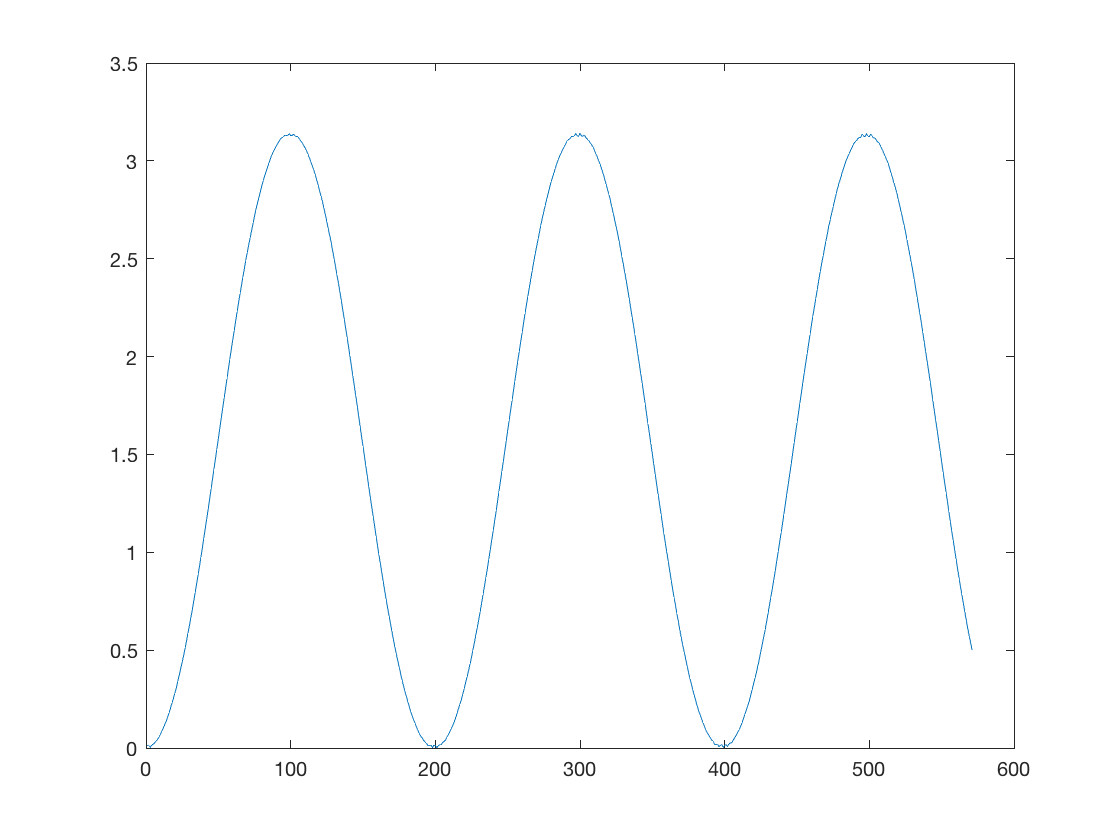
\includegraphics[width=0.89\textwidth]{E2000.png}
		\caption*{\small Figure 13(f), $\vec{\omega} = \vec{\omega_0}, \vec{\Omega} = {2}\vec{\Omega_0}$}
	\end{minipage}
\end{figure}


Observe that any two graphs in the same column are identical. That is to say, as long as the product of the angular velocity of the earth and that of the gyroscope is constant, the oscillating period of the axis would remain unchanged. Hence it must be that the two angular velocities enter the expression of oscillating period as a product. This result confirms the analytic derivation. See next section for further discussion.

\textbf{Remark:} Observe that when the gyrocompass settles down, the gyroscope is rotating in the same direction as the earth (i.e. viewed from the north, both the earth and the gyroscope are rotating counterclockwise). Although detailed analysis of how the gyroscope would navigate itself can be done, a more intuitive and ingenious explanation is the following. Suppose the gyrocompass is put at the equator, for simplicity. If we view the gyroscope and the earth together as a system, the total angular momentum should be conservative. In this case, the total angular momentum is the sum of the two angular momentum vectors from the earth and the gyroscope. At steady state the two vectors are parallel and are pointing to the same direction (i.e. north). Now if we manually invert the gyroscope's axis, making its angular momentum vector pointing south, then the two vectors are pointing at opposite directions. Due to the fact that their sum is constant, it must be that the magnitude of the earth's angular momentum becomes larger, or, the earth is rotating faster. A faster rotating earth possesses a higher kinetic energy, so work to the system is down by our action of inverting the gyroscope's axis. At equilibrium the system must operate under the lowest energy level. Hence the earth would slow down its speed, do work to the gyroscope, and finally invert it back so that the gyroscope's angular momentum vector is again pointing north, while during the whole process the sum of these two angular momentum vectors remain unchanged.

\section{Future studies}
\hspace{5mm} We haven't had time to fully investigate how the friction on the track will quantitatively influence the performance of a gyrocompass. In this \href{https://github.com/zeshunzong/A_series_of_experiments_based_on_gyroscope/blob/master/paper/gyrocompass_peskin.pdf}{\textbf{notes}} at \url{https://github.com/zeshunzong/A_series_of_experiments_based_on_gyroscope/blob/master/paper/gyrocompass_peskin.pdf}, Peskin shows that with some wisely chosen level of friction, oscillation can be gradually damped down and finally the axis of the gyroscope will stably points to the north. Analytic derivation is given in this notes, and in the future, we plan to verify this result using our model.




\section{Acknowledgement}

\hspace{5mm} We would like to show our gratitude to our mentor Professor Charles S. Peskin for his great guidance and encouragement. We would also like to present special thanks to Dr. Charles Puelz. He provides insightful advice to our model and essential help in code implementation.

All our code, notes, movies and graphs are available at \url{https://github.com/zeshunzong/A_series_of_experiments_based_on_gyroscope/tree/master/video}. Suggestions are welcomed.

\begin{comment}
\section{Appendix: Analysis of Gyrocompass's Motion}
\hspace{5mm} Let the center of mass of a gyroscope rotate with the earth, and let the axis of the gyroscope be constrained to lie in a locally horizontal	plane. Let $\vec{z}$ be a unit vector aligned with the earth's axis, pointing north, so that $\vec{\Omega z}$ is the angular velocity of the earth.

At the location of the gyroscope, let $$\{\vec{e}(t), \vec{n}(t), \vec{r}(t) \}$$ be an orthonormal set of vectors pointing east, north, and up (perpendicular to the tangent plane), respectively. Note that \begin{equation}
	\vec{z} \cdot \vec{e}(t) = 0, \vec{z} \cdot \vec{n}(t) = \cos(\theta), \vec{z} \cdot \vec{r}(t) = \sin(\theta),
\end{equation}
where $\theta$ is the latitude of the gyroscope.

Since $\vec{e}(t), \vec{n}(t), \vec{r}(t)$ are all rigidly attached to the rotating earth, they satisfy the same differential equation
\begin{equation}
	\frac{d \vec{v}(t)}{dt} = \vec{\Omega z} \times \vec{v}(t),
\end{equation}
where $\vec{v}$ denotes any of these vectors. Then if $\vec{w}$ is also any one of these vectors, we have
\begin{align*}
	\frac{d\vec{v}}{dt} \cdot &= \vec{\Omega} (\vec{z} \times \vec{v})\cdot \vec{w} \\
	&= \vec{\Omega} \vec{z} \cdot (\vec{v} \times \vec{w}).
\end{align*}
It follows that
\begin{align}
	\frac{d}{dt} \begin{bmatrix} \vec{e} \\ \vec{n} \\ \vec{r} \end{bmatrix} &= \vec{\Omega} \begin{bmatrix} 0 & \vec{z \cdot r} & -\vec{z \cdot n} \\ -\vec{z \cdot r} & 0 & \vec{z \cdot e} \\ \vec{z \cdot n} & -\vec{z \cdot e} & 0 \end{bmatrix} \begin{bmatrix} \vec{e} \\ \vec{n} \\ \vec{r} \end{bmatrix} \\
	&= \vec{\Omega} \begin{bmatrix} 0 & \sin(\theta) & -\cos(\theta) \\ -\sin(\theta) & 0 & 0 \\ \cos(\theta) & 0 & 0 \end{bmatrix} \begin{bmatrix} \vec{e} \\ \vec{n} \\ \vec{r} \end{bmatrix},
\end{align}
where the first equality follows from the fact that $\vec{e} \times \vec{n} = \vec{r},$ and so on.

We define $\vec{a}(t)$ to be the vector aligned with the axis of the gyroscope, and define $$\vec{b}(t) = \vec{r}(t) \times \vec{a}(t).$$ Since the axis is constrained to lie in the locally horizontal plane, we can write
\begin{equation}
	\vec{a}(t) = \cos(\phi(t)) \vec{e}(t) + \sin(\phi(t))\vec{n}(t),
\end{equation}
and
\begin{equation}
	\vec{b}(t) = -\sin(\phi(t)) \vec{e}(t) + \cos(\phi(t))\vec{n}(t).
\end{equation}
We seek to derive an equation that describes the motion for the angle $\phi(t).$

% below we do not use \vec. NEED to replace

Let $\vec{\omega} (t)$ be the angular velocity of the gyroscope. We can write it in the basis $\{\vec{a}(t), \vec{b}(t), \vec{r}(t)\}$ as
$$\vec{\omega}(t) = \vec{\omega}_{\vec{a}}(t)\vec{a}(t) + \vec{\omega}_{\vec{b}}(t) \vec{b}(t) + \vec{\omega}_{\vec{r}}(t) \vec{r}(t).$$

Since $\vec{a}$ moves rigidly with the material of the rotating gyroscope, it has the differential equation
\begin{equation}
	111
\end{equation}
\end{comment}
\begin{thebibliography}{9}

	\bibitem{gyrocom}
	Charles S. Peskin. (2018).
	Notes on gyrocompass.

	\bibitem{rbm}
	Charles Puelz. (2018).
	Matlab code about rigid body motion.




\end{thebibliography}

\end{document}
